\documentclass[12pt,a4paper]{article}

% ── packages ───────────────────────────────────────────────────────────────
\usepackage[utf8]{inputenc}
\usepackage[T1]{fontenc}
\usepackage[english]{babel}
\usepackage{graphicx}
\usepackage{booktabs}
\usepackage{amsmath}
\usepackage{hyperref}
\usepackage{geometry}
\usepackage{caption}
\usepackage{float}

\geometry{margin=2.5cm}

\title{Custom-WikiCS Graph Analysis -- Part 4\\[4pt]
\large Unified Advanced Analytics: Topic-Link Assortativity, Local Transitivity \& Community Similarity}
\author{}
\date{\today}

\begin{document}
\maketitle

% ═══════════════════════════════════════════════════════════════════════════
\section{Introduction}
% ═══════════════════════════════════════════════════════════════════════════

This fourth report unifies and extends the structural analyses performed in the
previous phases, now on the \textbf{cleaned} graph with isolated (degree-0) nodes
removed.  The Custom-WikiCS graph is a directed graph derived from Wikipedia
computer-science articles: each node represents an article, each directed edge
represents a hyperlink, and every node carries a 1024-dimensional embedding vector
produced by the \textbf{BAAI/bge-m3} sentence-embedding model.

The analyses covered in this report include:
\begin{enumerate}
    \item Removal of isolated nodes and graph pre-processing.
    \item Degree distribution analysis and log-log power-law assessment.
    \item Degree assortativity coefficient.
    \item Topic-link assortativity: linked vs.\ random pair similarity using
          Cosine Similarity, Pearson Correlation, and Euclidean Distance.
    \item Local transitivity (clustering coefficient) distribution.
    \item Degree vs.\ similarity metrics scatter plots.
    \item Local transitivity vs.\ cosine similarity scatter plots.
    \item Connected component size distributions.
    \item Centrality measures: Degree, Betweenness, Closeness, PageRank, Eigenvector.
    \item Community detection: Louvain and Infomap with modularity and size statistics.
    \item Intra-community vs.\ inter-community similarity analysis with box plots.
    \item Node degree range vs.\ average neighbor similarity box plot.
\end{enumerate}

\begin{itemize}
    \item \textbf{Nodes (cleaned):} 11\,367
    \item \textbf{Directed edges:} 291\,039
    \item \textbf{Undirected edges:} 216\,123
    \item \textbf{Isolated nodes removed:} 334 (from 11\,701)
\end{itemize}

% ═══════════════════════════════════════════════════════════════════════════
\section{Data Pre-processing: Isolated Node Removal}
% ═══════════════════════════════════════════════════════════════════════════

All isolated nodes (degree~$= 0$) were identified and removed prior to analysis.
These nodes represent articles that neither link to nor are linked from any other
article, contributing no structural information to the graph.

\begin{table}[H]
\centering
\caption{Graph statistics before and after cleaning.}
\label{tab:cleaning}
\begin{tabular}{lrrr}
\toprule
\textbf{Metric} & \textbf{Original Graph} & \textbf{Cleaned Graph} & \textbf{Reduction} \\
\midrule
Nodes & 11\,701 & 11\,367 & 334 (2.85\%) \\
Directed Edges & 291\,039 & 291\,039 & 0 (0.00\%) \\
Undirected Edges & 216\,123 & 216\,123 & 0 (0.00\%) \\
\bottomrule
\end{tabular}
\end{table}

The removal of \textbf{334 isolated nodes} leaves 11\,367 active nodes.  The edge
count is unchanged because isolated nodes, by definition, carry no edges.  All
subsequent analyses in this report are performed on this cleaned graph.

% ═══════════════════════════════════════════════════════════════════════════
\section{Degree Distribution}
% ═══════════════════════════════════════════════════════════════════════════

Figure~\ref{fig:degree_dist} shows the total-degree, in-degree, and out-degree
distributions on the cleaned graph.

\begin{figure}[H]
    \centering
    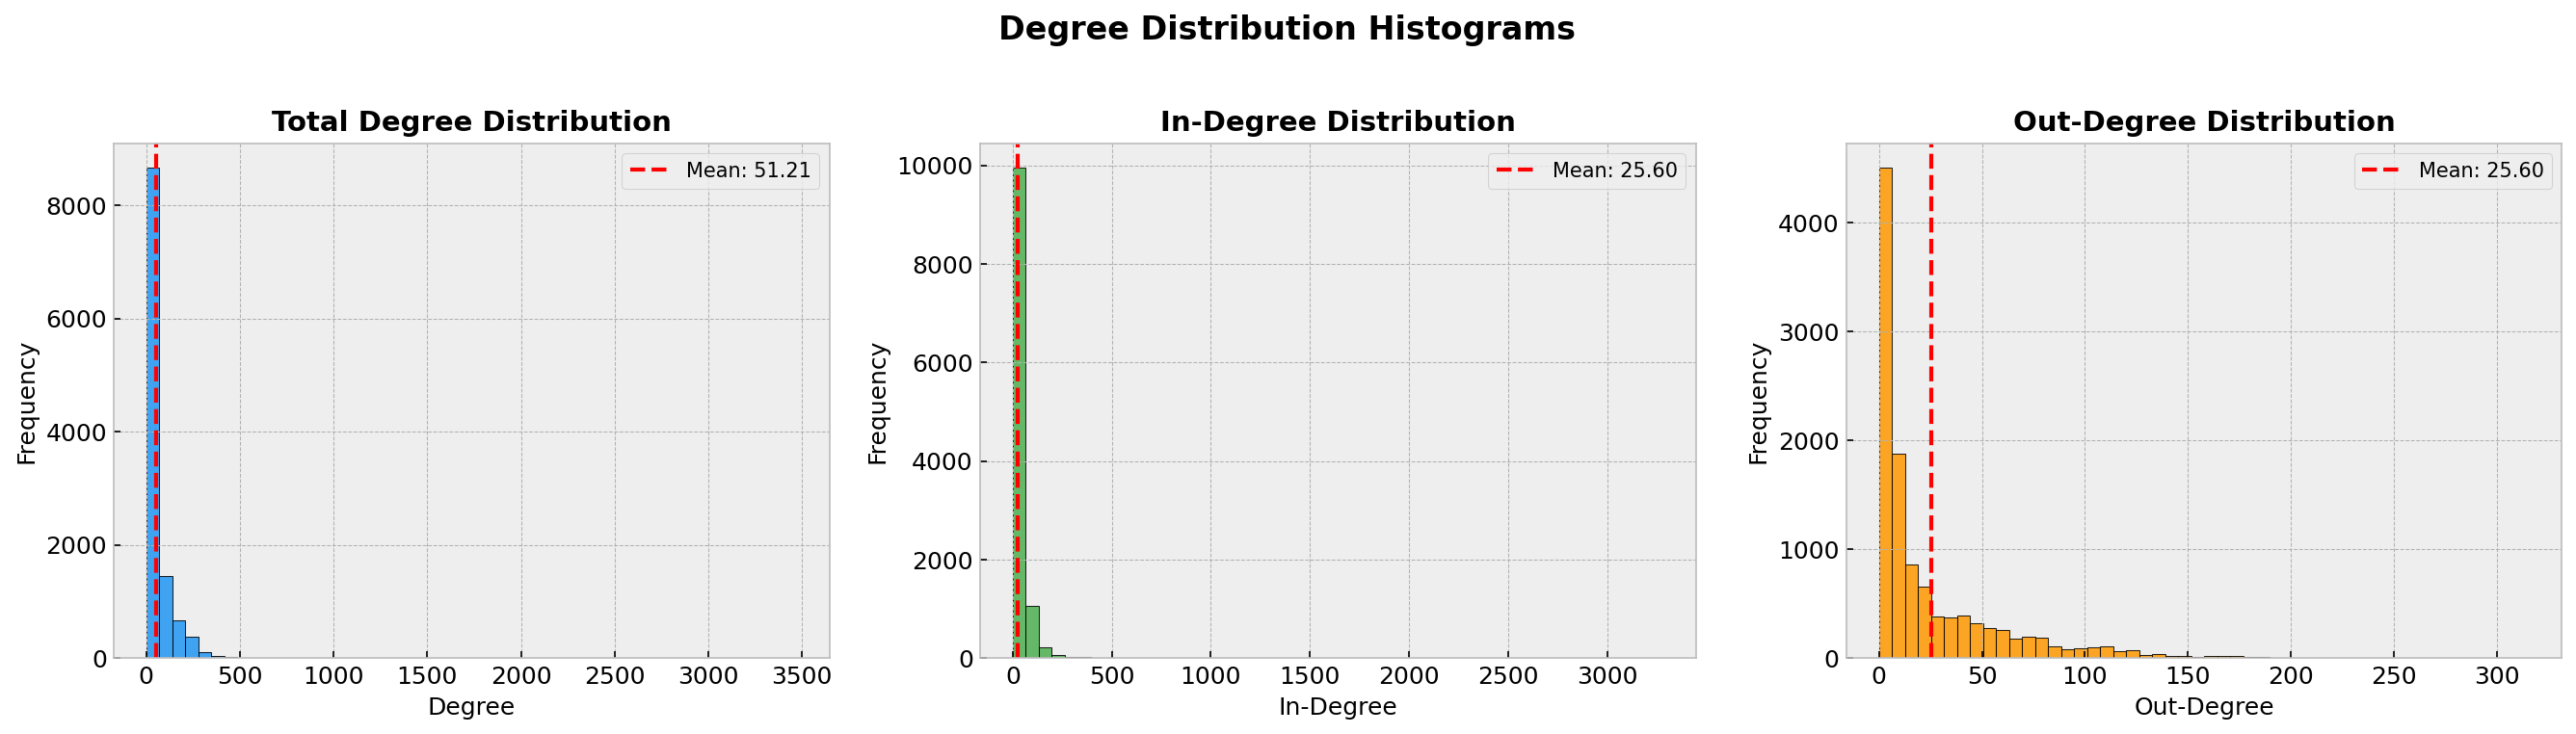
\includegraphics[width=\textwidth]{img-4/degree-distribution.png}
    \caption{Total, In, and Out degree distributions on the cleaned graph.}
    \label{fig:degree_dist}
\end{figure}

\begin{table}[H]
\centering
\caption{Degree statistics for the cleaned graph.}
\label{tab:degree_stats}
\begin{tabular}{lrrrr}
\toprule
 & \textbf{Min} & \textbf{Max} & \textbf{Mean} & \textbf{Median} \\
\midrule
Total Degree & 1 & 3\,474 & 51.21 & 16 \\
In-Degree    & 0 & 3\,283 & 25.60 & 4 \\
Out-Degree   & 0 & 316    & 25.60 & 10 \\
\bottomrule
\end{tabular}
\end{table}

All three distributions are heavily right-skewed.  The total-degree histogram is
dominated by a tall first bin (degree~$<50$), with a long tail extending to
3\,474.  The in-degree distribution is the most extreme: the majority of nodes
have fewer than 50 incoming links, while a handful of hub articles attract over
3\,000 incoming links.  The out-degree distribution is comparatively compact
(max~316) with a smoother decay, suggesting that articles tend to link out to a
limited number of targets regardless of how many links they receive.

\subsection{Log--Log Scale}

Figure~\ref{fig:degree_loglog} presents the total-degree distribution on log--log
axes to assess power-law behaviour.

\begin{figure}[H]
    \centering
    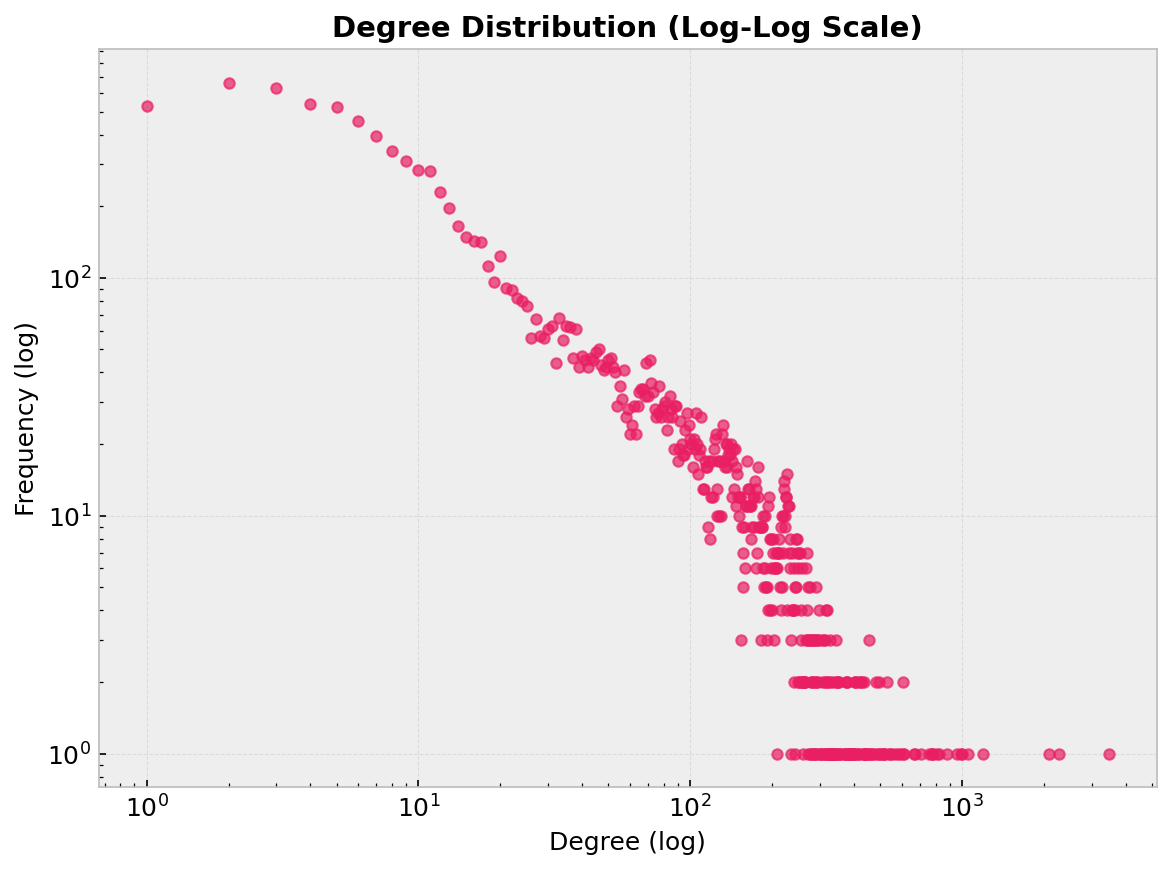
\includegraphics[width=0.65\textwidth]{img-4/degree-log-log.png}
    \caption{Degree distribution on log--log scale.}
    \label{fig:degree_loglog}
\end{figure}

The approximately linear relationship on log--log axes from degree~1
(frequency $\sim$4\,000) down to degree $\sim$3\,500 (frequency~1) is consistent
with a power-law--like (scale-free) degree distribution, a hallmark of many
real-world networks including the World Wide Web.

% ═══════════════════════════════════════════════════════════════════════════
\section{Degree Assortativity}
% ═══════════════════════════════════════════════════════════════════════════

The \emph{degree assortativity coefficient}~$r$ measures whether high-degree nodes
tend to connect to other high-degree nodes (\emph{assortative}, $r>0$) or to
low-degree nodes (\emph{disassortative}, $r<0$).

\[
    r = -0.0918
\]

The negative coefficient indicates that the cleaned graph is
\textbf{disassortative}: high-degree nodes tend to connect to low-degree nodes.
This is consistent with the typical structure of information networks (e.g.,
Wikipedia), where a few highly-linked hub articles reference many less-popular
articles.

% ═══════════════════════════════════════════════════════════════════════════
\section{Topic-Link Assortativity}
% ═══════════════════════════════════════════════════════════════════════════

To assess whether linked articles are also \emph{topically similar}, we compare
the BAAI/bge-m3 embedding vectors of connected node pairs against those of
randomly sampled (unconnected) pairs using three metrics: Cosine Similarity,
Pearson Correlation, and Euclidean Distance.

\begin{figure}[H]
    \centering
    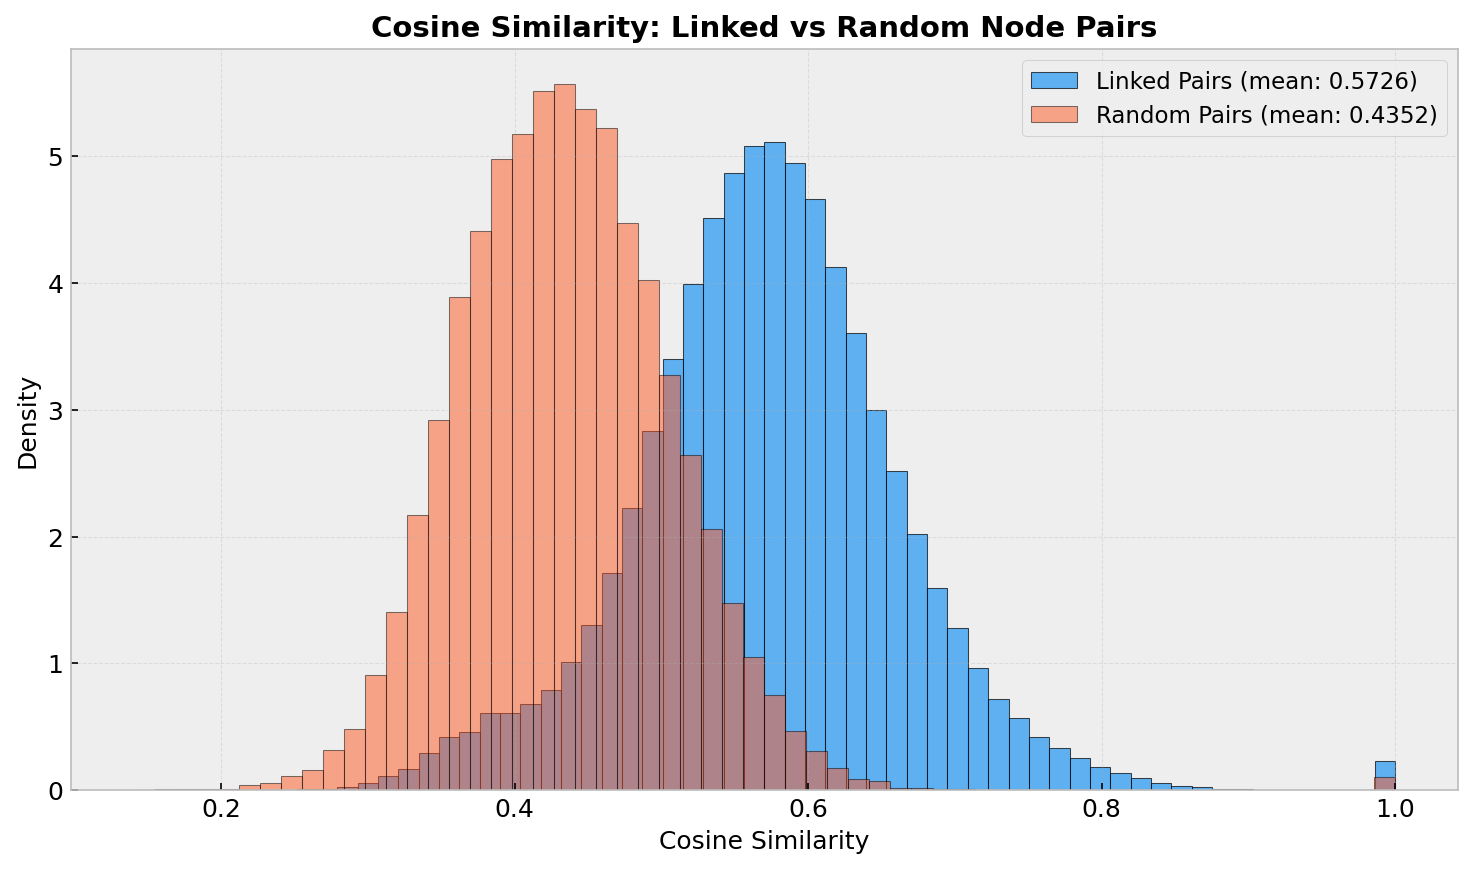
\includegraphics[width=0.8\textwidth]{img-4/cosine-similarity-assortativity.png}
    \caption{Cosine similarity distribution: linked vs.\ random node pairs.}
    \label{fig:cosine}
\end{figure}

Linked pairs exhibit a cosine similarity of $0.5726$ on average, roughly
$+0.14$ higher than the random baseline ($0.4352$).  This confirms that connected
articles tend to be topically more similar than arbitrary pairs.

\begin{figure}[H]
    \centering
    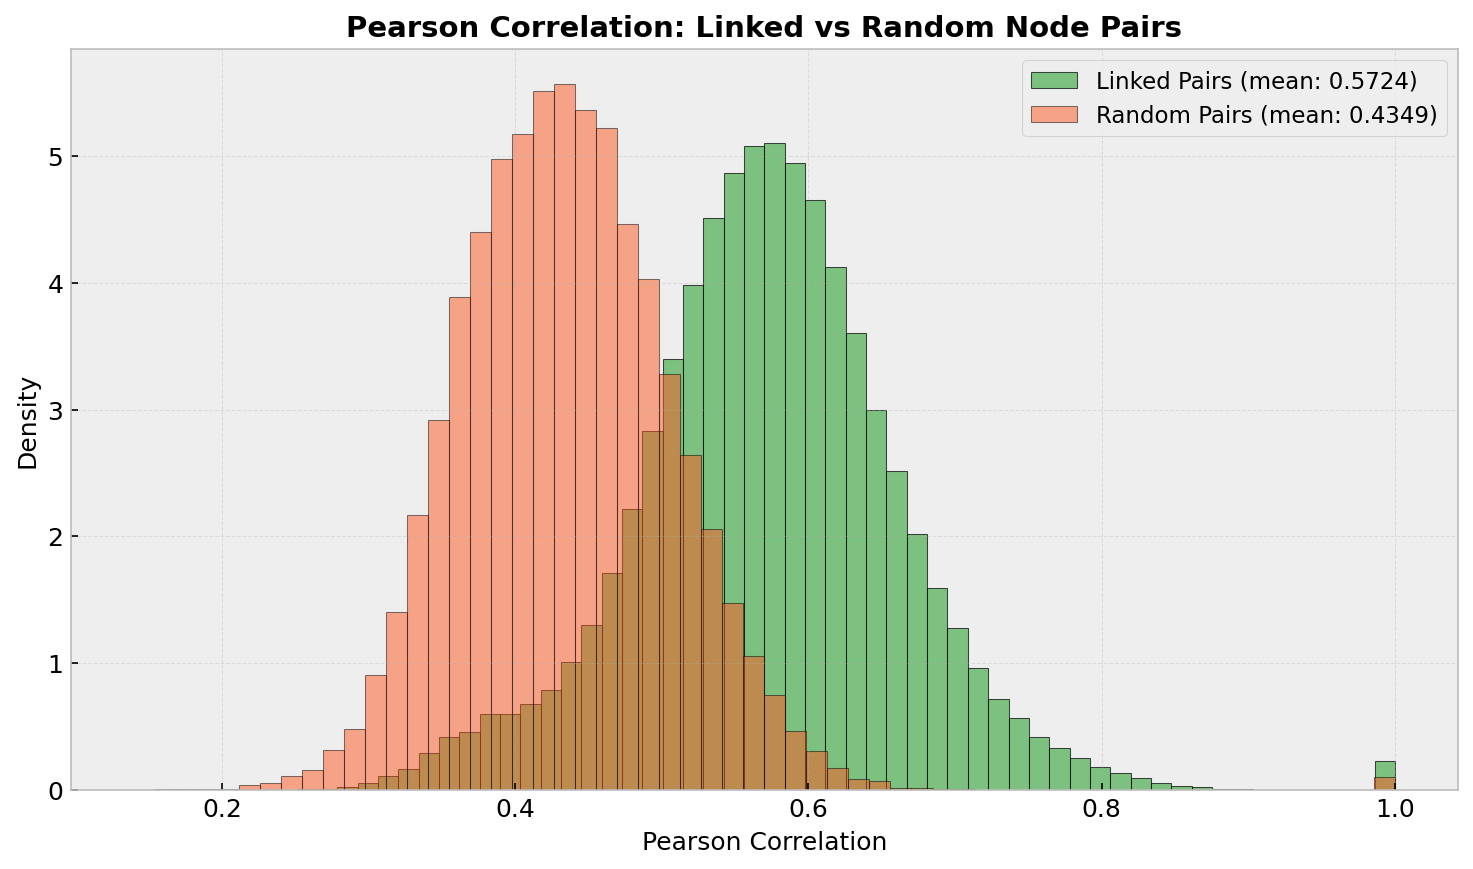
\includegraphics[width=0.8\textwidth]{img-4/pearson-correlation-assortativity.png}
    \caption{Pearson correlation distribution: linked vs.\ random node pairs.}
    \label{fig:pearson}
\end{figure}

Pearson correlation mirrors the cosine similarity pattern almost exactly
($0.5724$ vs.\ $0.4349$), as expected for $\ell_2$-normalised vectors.

\begin{figure}[H]
    \centering
    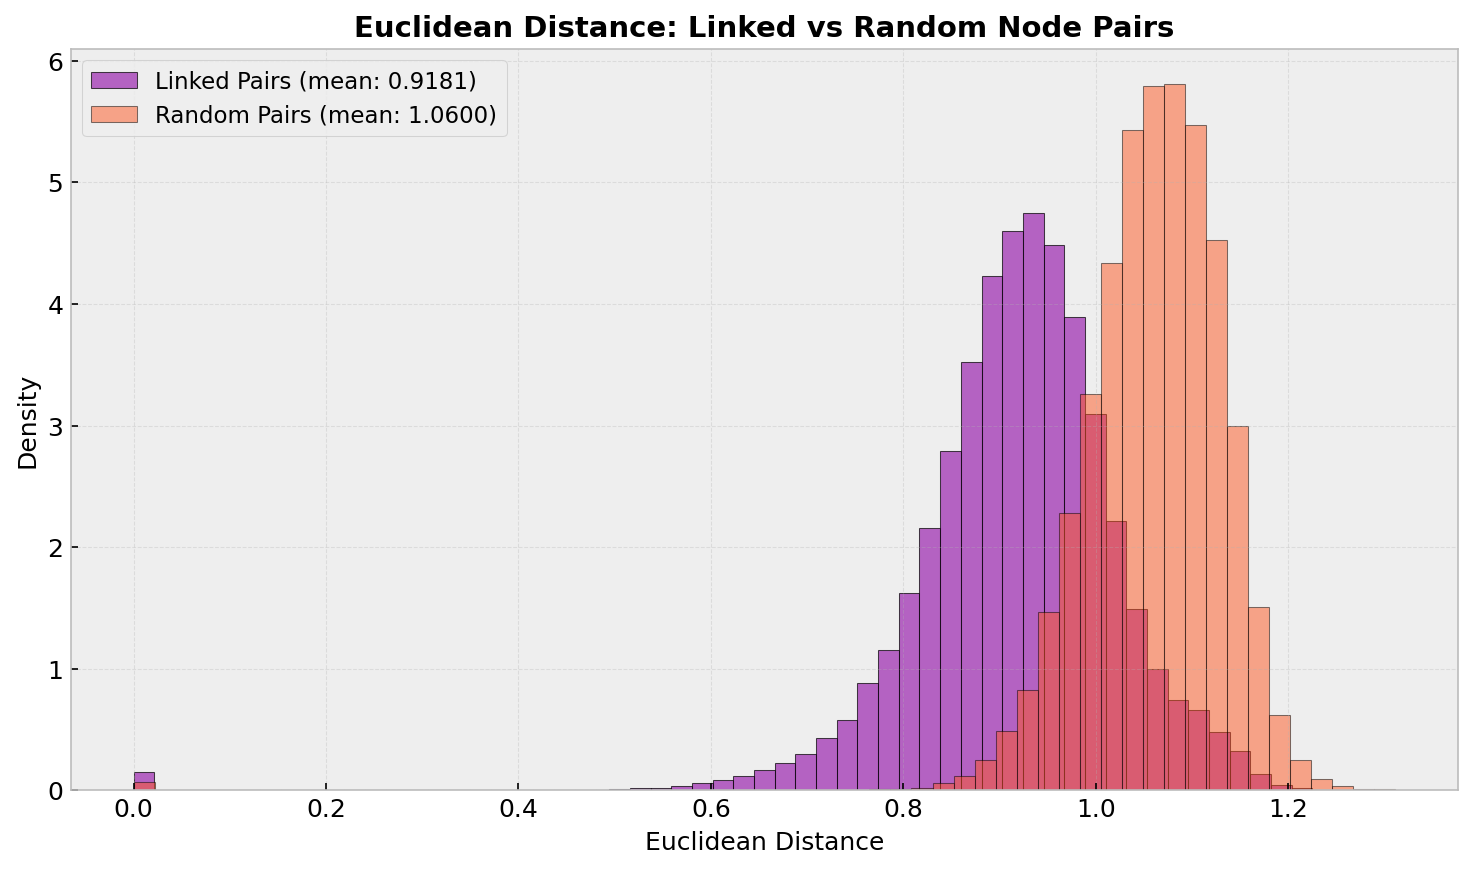
\includegraphics[width=0.8\textwidth]{img-4/euclidean-distance-assortativity.png}
    \caption{Euclidean distance distribution: linked vs.\ random node pairs.}
    \label{fig:euclidean}
\end{figure}

For Euclidean distance, linked pairs are on average closer ($0.9181$) than random
pairs ($1.0600$), a difference of $-0.1419$.  The normalised embedding space
compresses all distances into a narrow range, so the two distributions overlap
substantially, yet the systematic shift confirms topical coherence of links.

\begin{table}[H]
\centering
\caption{Topic-link assortativity summary.}
\label{tab:topic_link}
\begin{tabular}{lccccc}
\toprule
\textbf{Metric} & \textbf{Linked Mean} & \textbf{Linked Std} & \textbf{Random Mean} & \textbf{Random Std} & \textbf{Diff} \\
\midrule
Cosine Similarity    & 0.5726 & 0.0901 & 0.4352 & 0.0724 & +0.1374 \\
Pearson Correlation  & 0.5724 & 0.0902 & 0.4349 & 0.0725 & +0.1375 \\
Euclidean Distance    & 0.9181 & 0.1089 & 1.0600 & 0.0773 & $-0.1419$ \\
\bottomrule
\end{tabular}
\end{table}

% ═══════════════════════════════════════════════════════════════════════════
\section{Local Transitivity (Clustering Coefficient)}
% ═══════════════════════════════════════════════════════════════════════════

The \emph{local clustering coefficient} (transitivity) of a node~$v$ measures the
fraction of $v$'s neighbour pairs that are also connected to each other.  High
values indicate that $v$ sits inside a tightly-knit cluster.

\begin{figure}[H]
    \centering
    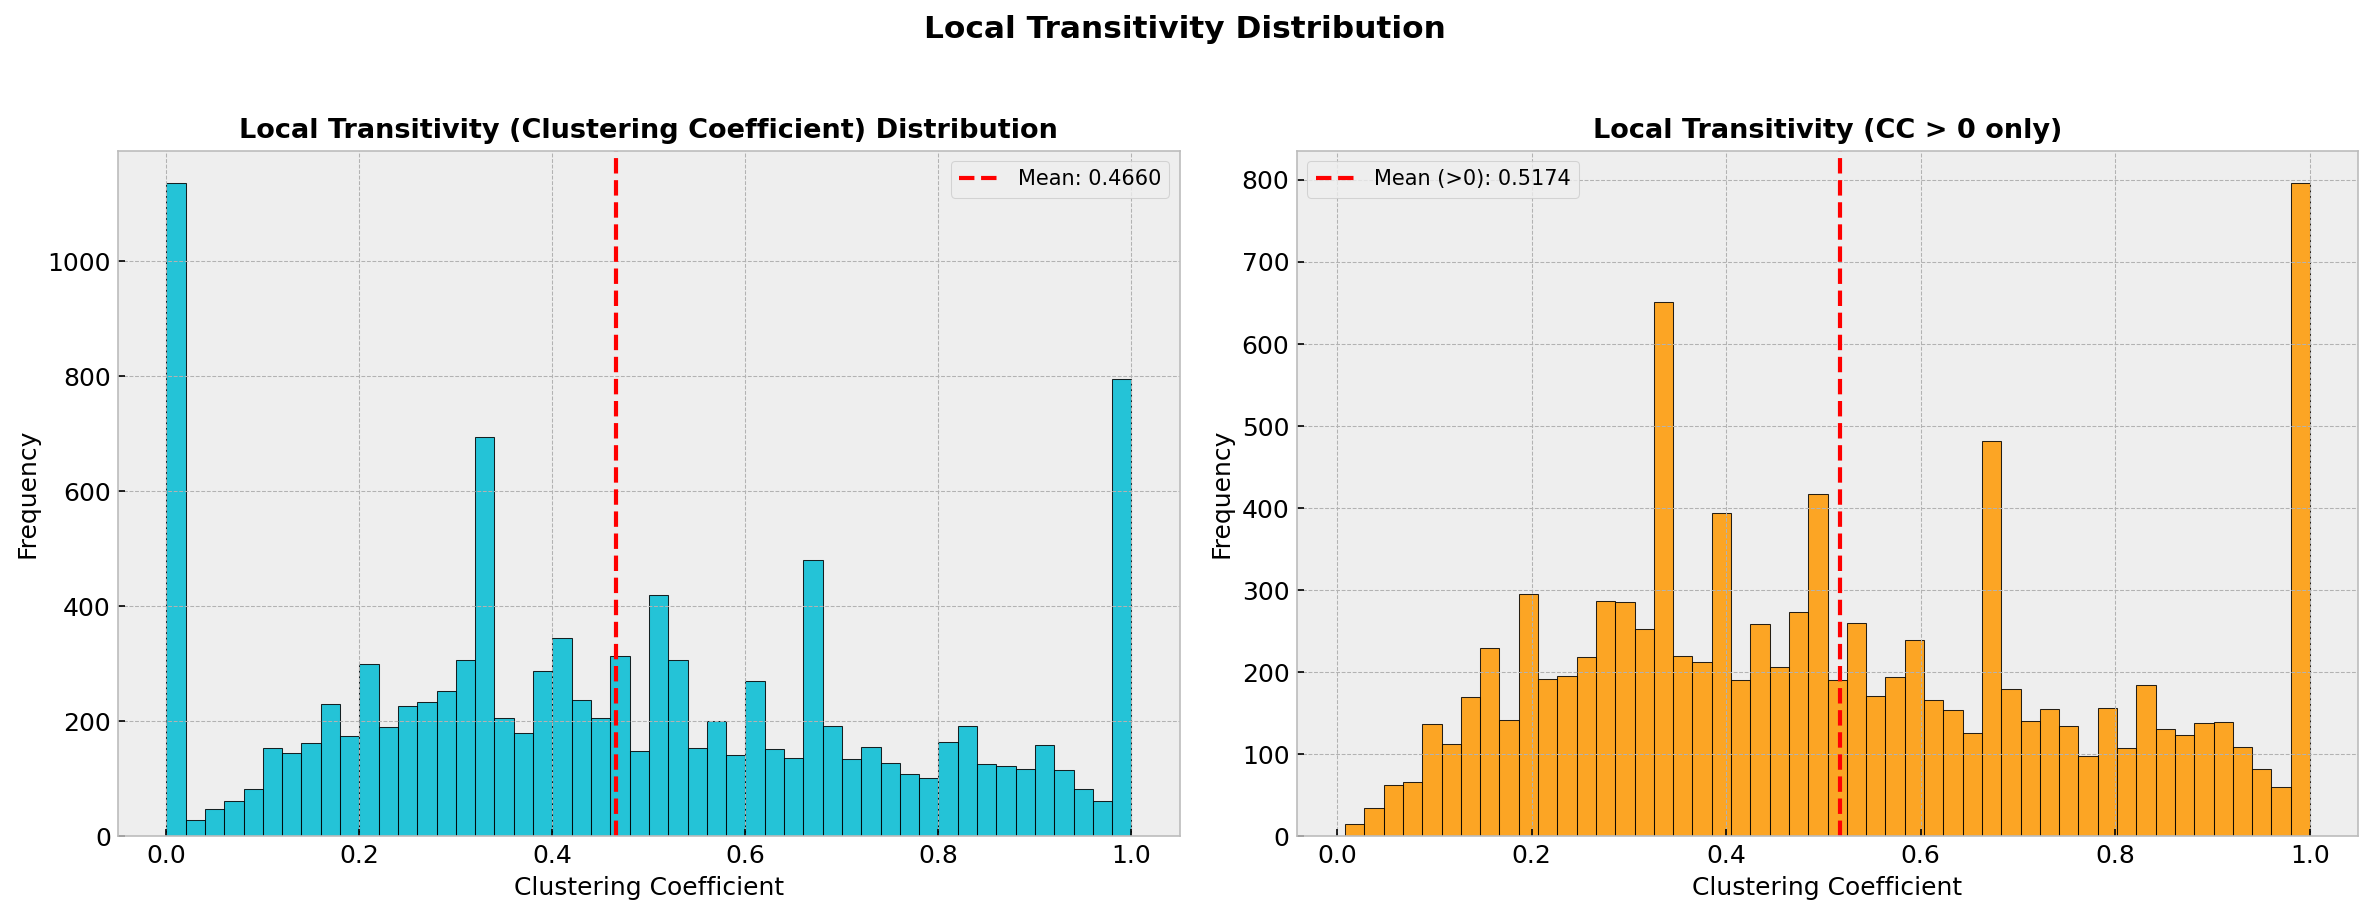
\includegraphics[width=\textwidth]{img-4/local-transitivity-distribution.png}
    \caption{Local transitivity distribution: all nodes (left) and nodes with
             CC~$>0$ (right).  Red dashed line marks the mean.}
    \label{fig:transitivity}
\end{figure}

\begin{table}[H]
\centering
\caption{Local transitivity statistics.}
\label{tab:cc_stats}
\begin{tabular}{lr}
\toprule
\textbf{Statistic} & \textbf{Value} \\
\midrule
Mean CC            & 0.4660 \\
Median CC          & 0.4402 \\
Min CC             & 0.0000 \\
Max CC             & 1.0000 \\
Std CC             & 0.2931 \\
Global Transitivity & 0.2623 \\
\bottomrule
\end{tabular}
\end{table}

The left histogram shows a prominent spike at CC~$=0$, reflecting nodes whose
neighbours are not connected to each other (typically leaf or path nodes).
When these zero-CC nodes are excluded (right panel), the distribution becomes
roughly uniform across $(0,1)$ with a multimodal shape.  The mean local
clustering coefficient ($0.4660$) and the notably lower global transitivity
($0.2623$) indicate that triangles are relatively scarce at the global level,
even though many individual nodes sit in dense local neighbourhoods.

% ═══════════════════════════════════════════════════════════════════════════
\section{Degree vs.\ Similarity Metrics}
% ═══════════════════════════════════════════════════════════════════════════

To investigate how topical similarity between linked articles relates to the
connectivity of the endpoints, Figure~\ref{fig:deg_sim_metrics} plots each of the
three similarity metrics (Cosine Similarity, Euclidean Distance, Pearson
Correlation) against the degree of the source and target nodes of every edge.

\begin{figure}[H]
    \centering
    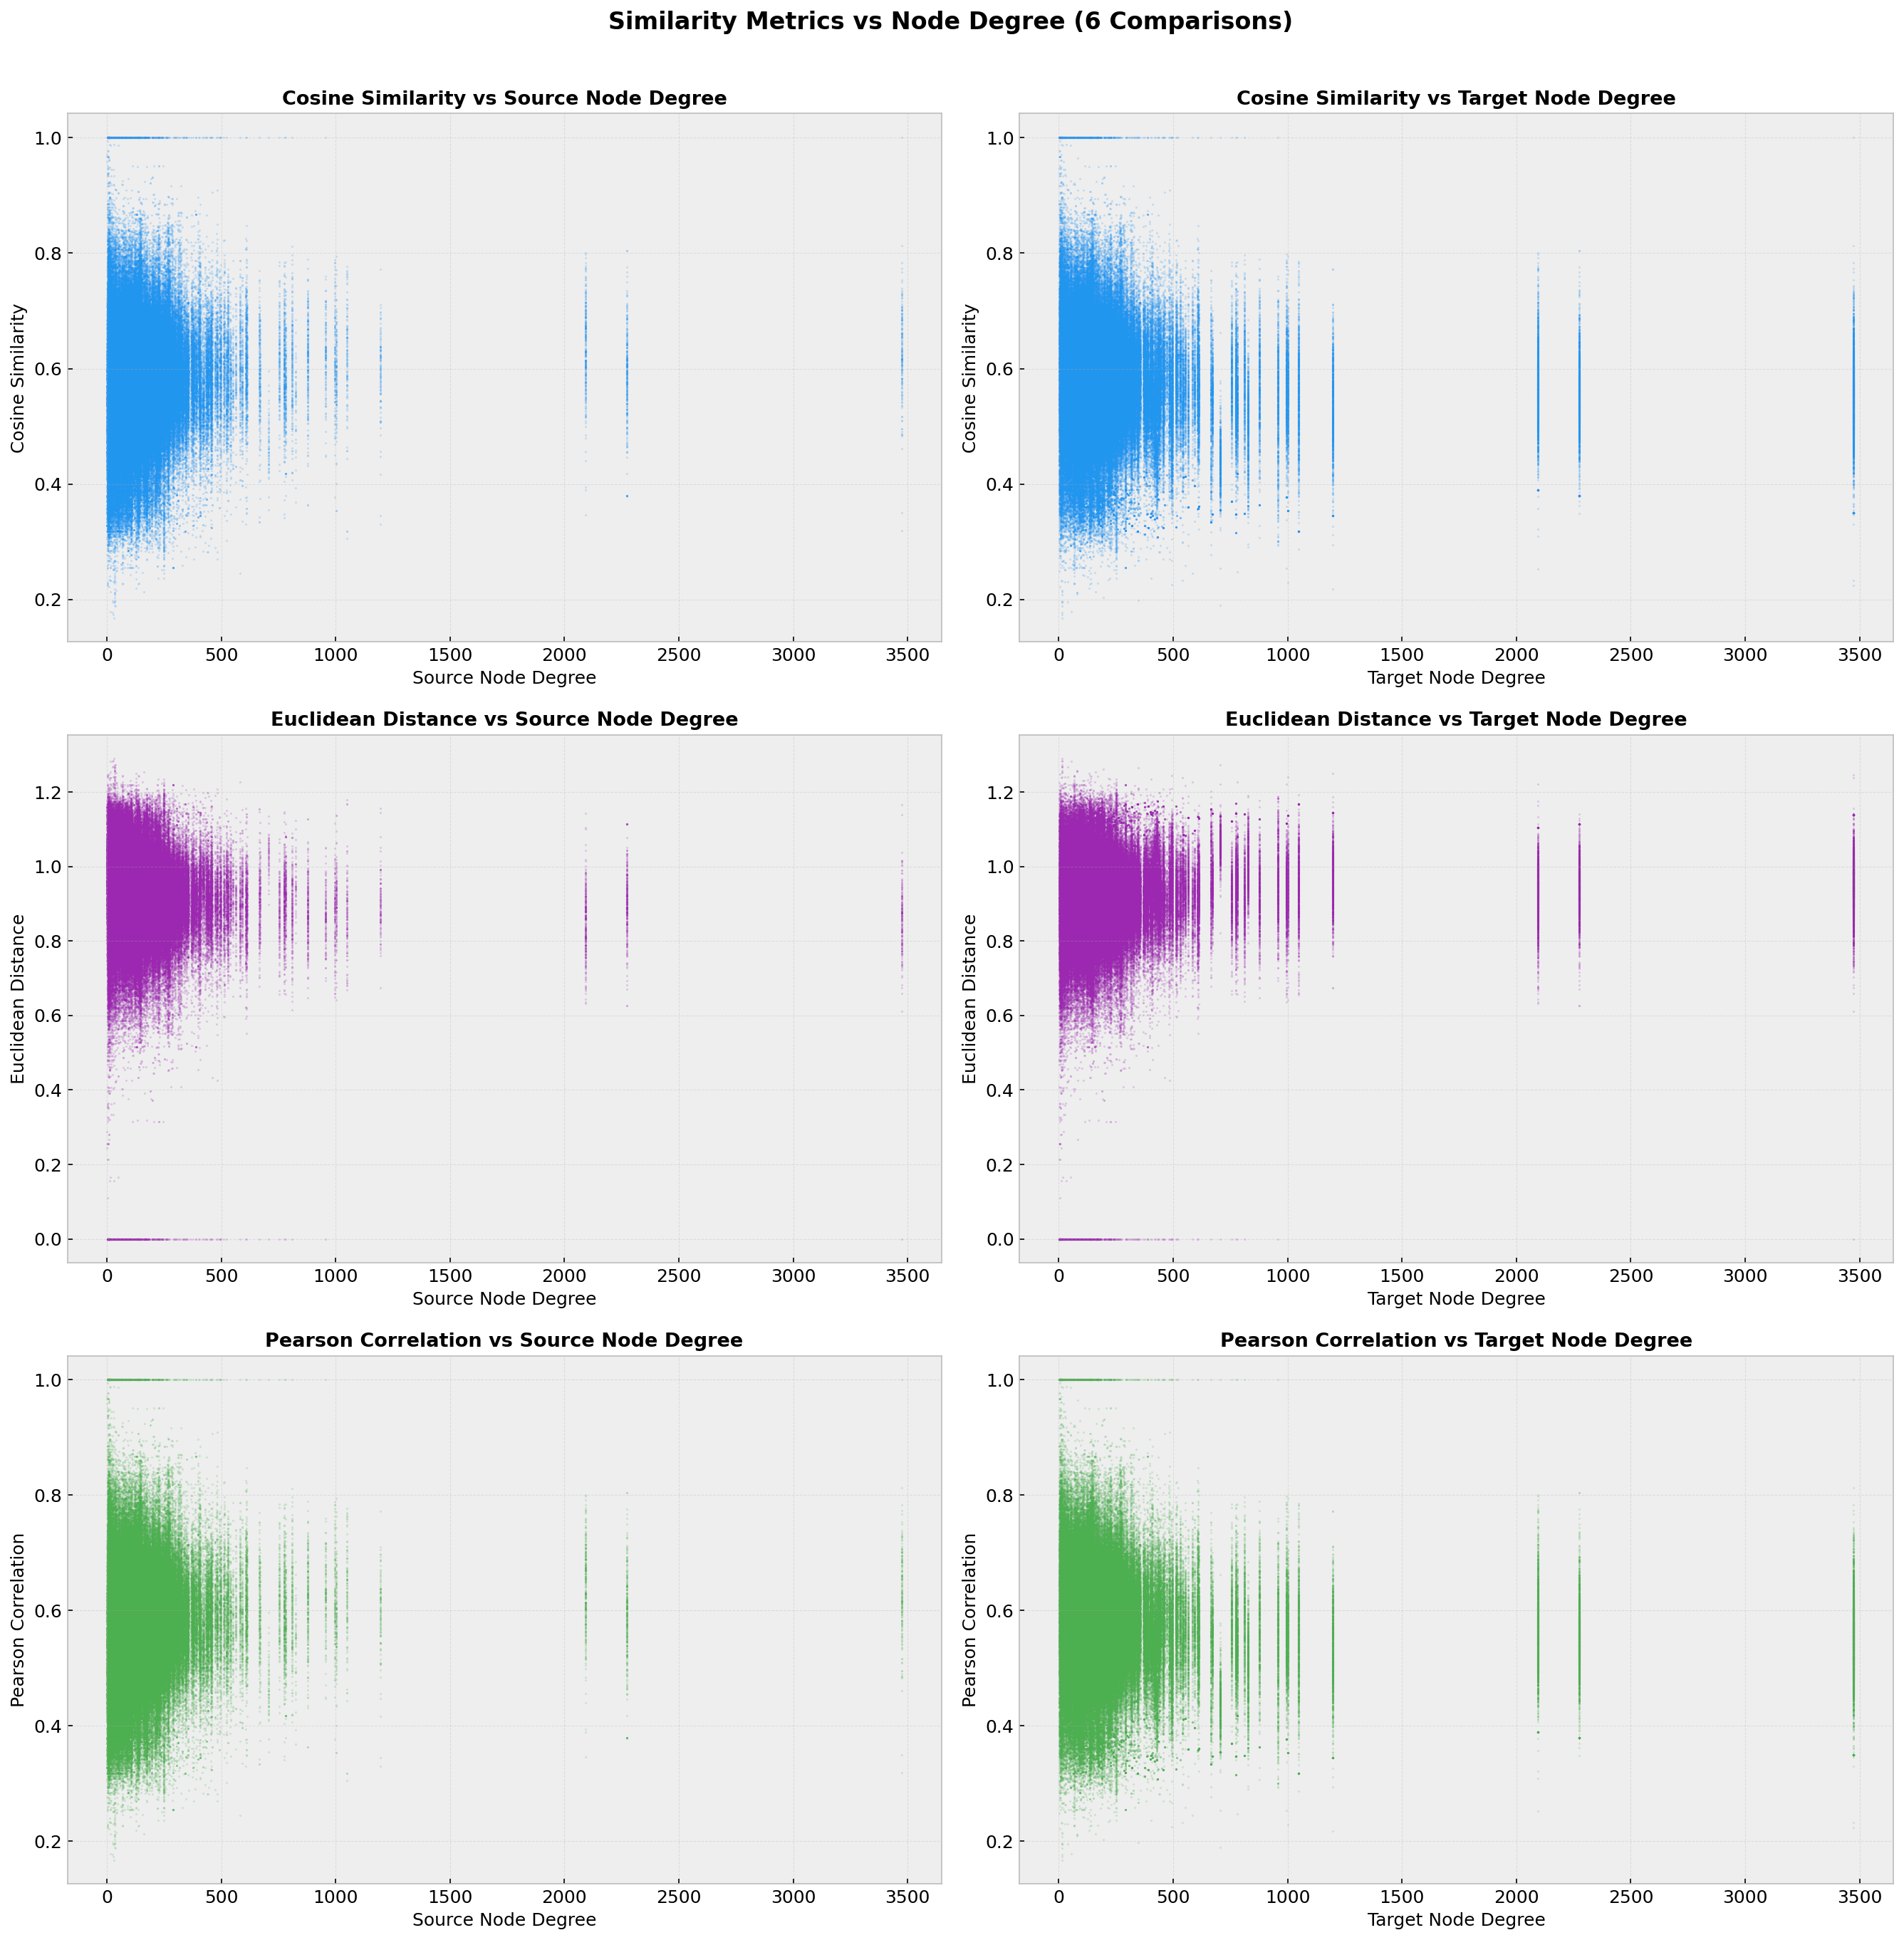
\includegraphics[width=\textwidth]{img-4/degree-vs-similarity-metrics.png}
    \caption{Similarity metrics vs.\ node degree for source and target nodes.
             Each row corresponds to a different metric.}
    \label{fig:deg_sim_metrics}
\end{figure}

Key observations:
\begin{itemize}
    \item For low-degree nodes (degree~$<500$) the similarity values span a wide
          range---cosine similarity stretches from $\sim$0.2 to 1.0 and Euclidean
          distance from $\sim$0.0 to 1.2.
    \item As degree increases beyond $\sim$500, the spread narrows markedly and
          converges toward the global mean ($\sim$0.57 for cosine, $\sim$0.92 for
          Euclidean).  Hub nodes connect to many diverse articles, so their
          per-edge similarity regresses toward the population average.
    \item A conspicuous horizontal band at Euclidean distance $\approx 0$ (cosine
          $\approx 1.0$) corresponds to near-duplicate or very closely related
          article pairs.
    \item The Pearson correlation panels mirror the cosine panels almost exactly,
          confirming effective $\ell_2$-normalisation of the bge-m3 embeddings.
    \item Patterns are largely symmetric between source and target degree,
          consistent with topical similarity being an undirected property.
\end{itemize}

% ═══════════════════════════════════════════════════════════════════════════
\section{Local Transitivity vs.\ Cosine Similarity}
% ═══════════════════════════════════════════════════════════════════════════

Figure~\ref{fig:trans_sim} examines the relationship between cosine similarity
of connected pairs and the local clustering coefficient of the source and target
nodes.

\begin{figure}[H]
    \centering
    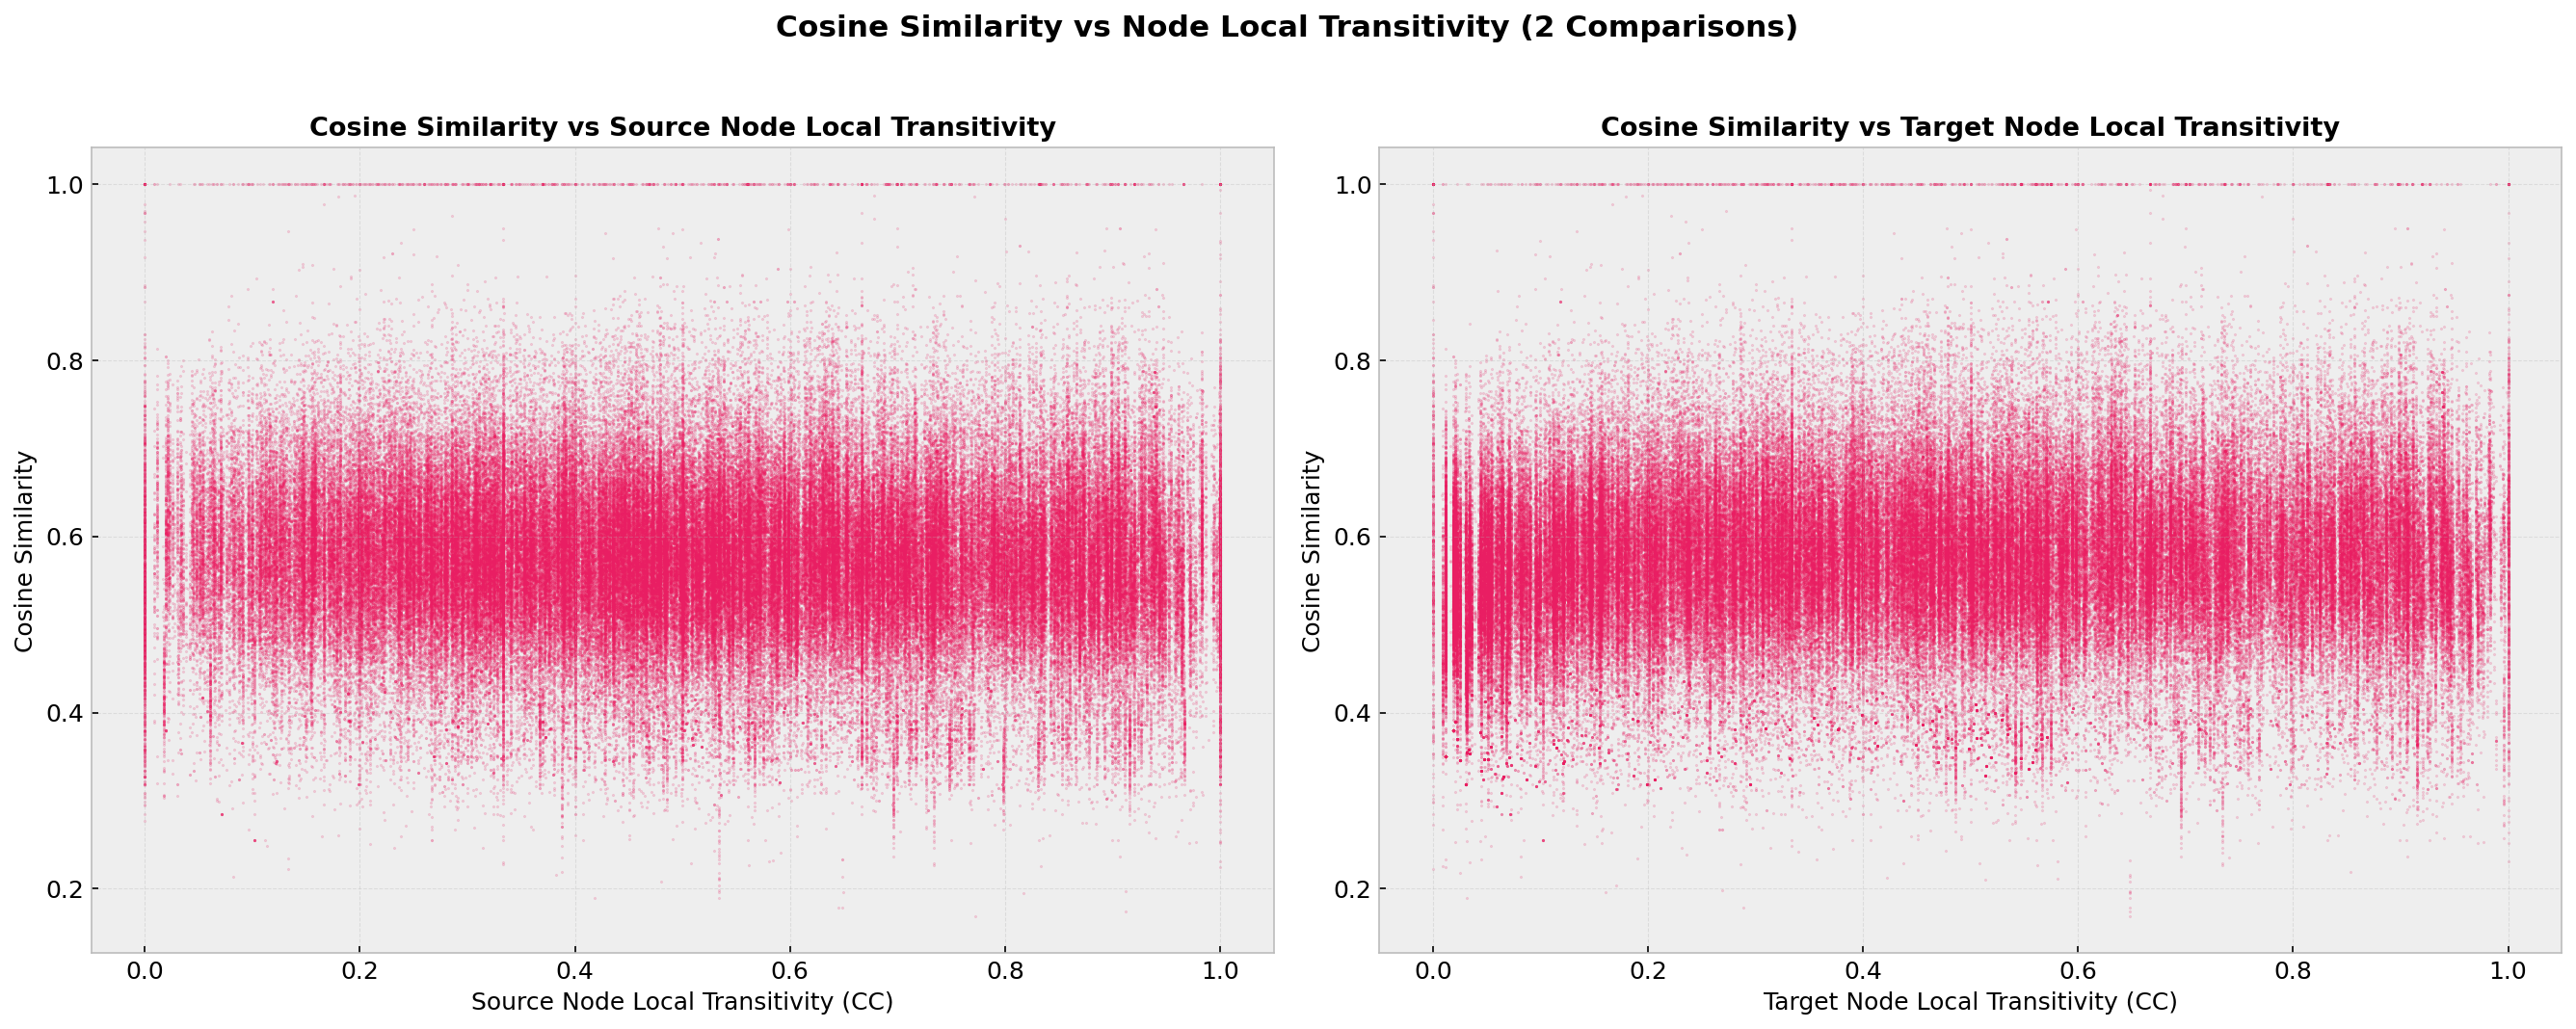
\includegraphics[width=\textwidth]{img-4/transitivity-vs-similarity.png}
    \caption{Cosine similarity vs.\ local transitivity of the source node (left)
             and target node (right).}
    \label{fig:trans_sim}
\end{figure}

Both scatter plots display a dense, horizontally uniform cloud with cosine
similarity concentrated in the $0.4$--$0.7$ band.  Unlike some other embedding
models, there is \emph{no clear positive or negative trend} between local
transitivity and cosine similarity: the cloud density remains essentially flat
from CC~$=0$ to CC~$=1$.  A thin horizontal line at cosine~$=1.0$ spans all CC
values, corresponding to near-duplicate article pairs.  This indicates that,
under the BAAI/bge-m3 representation, local clustering structure is largely
orthogonal to topical similarity.

% ═══════════════════════════════════════════════════════════════════════════
\section{Connected Component Analysis}
% ═══════════════════════════════════════════════════════════════════════════

A \emph{weakly connected component} (WCC) ignores edge direction; a
\emph{strongly connected component} (SCC) requires a directed path in both
directions.

\begin{figure}[H]
    \centering
    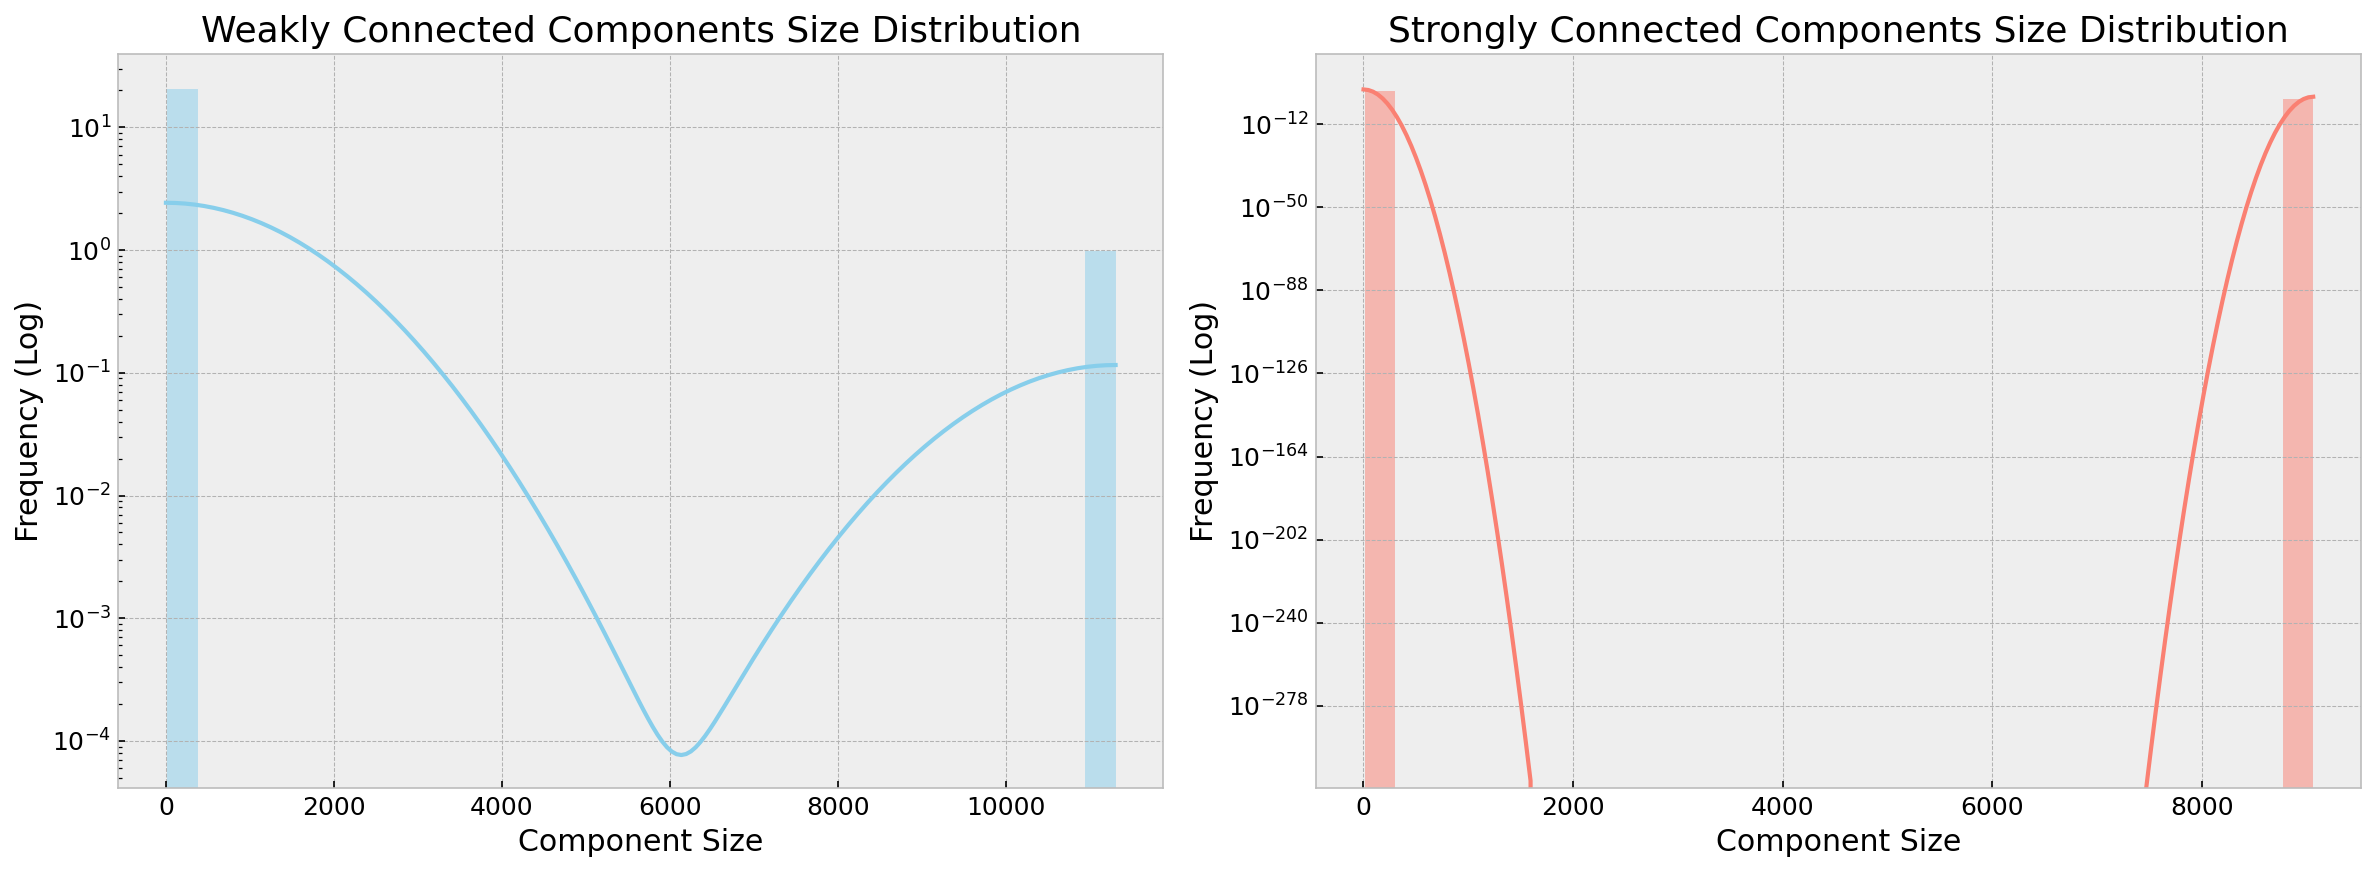
\includegraphics[width=\textwidth]{img-4/component-distributions.png}
    \caption{Component size distributions (log scale): Weakly Connected (left)
             and Strongly Connected (right).}
    \label{fig:components}
\end{figure}

\begin{table}[H]
\centering
\caption{Connected component statistics for the cleaned graph.}
\label{tab:components}
\begin{tabular}{lrrrl}
\toprule
\textbf{Metric} & \textbf{Count} & \textbf{Largest} & \textbf{Coverage} \\
\midrule
Weakly Connected Components    & 22     & 11\,311 nodes & 99.5\% \\
Strongly Connected Components  & 2\,176 & 9\,062 nodes  & 79.7\% \\
\bottomrule
\end{tabular}
\end{table}

The cleaned graph contains only \textbf{22 weakly connected components}, with
the largest WCC covering 11\,311 of the 11\,367 nodes ($99.5\%$).  This reveals
that virtually all non-isolated articles are mutually reachable when edge
direction is ignored.  The number of SCCs rises to 2\,176, and the largest SCC
encompasses 9\,062 nodes ($79.7\%$).  The gap between WCC and SCC coverage
($99.5\%$ vs.\ $79.7\%$) reflects a substantial directed periphery: nodes that
are reachable from the giant SCC but do not link back, forming an in-component
or out-component around the directed core.

% ═══════════════════════════════════════════════════════════════════════════
\section{Centrality Measures}
% ═══════════════════════════════════════════════════════════════════════════

Five centrality metrics were computed: Degree and PageRank on the directed graph;
Betweenness, Closeness, and Eigenvector on the undirected version.

\begin{table}[H]
\centering
\caption{Centrality statistics for the cleaned graph (11\,367 nodes).}
\label{tab:centrality}
\begin{tabular}{lrrrr}
\toprule
\textbf{Metric} & \textbf{Min} & \textbf{Max} & \textbf{Mean} & \textbf{Std} \\
\midrule
Degree Centrality      & 0.000088 & 0.305648 & 0.004505 & 0.007880 \\
Betweenness Centrality & 0.000000 & 0.215722 & 0.000176 & 0.002481 \\
Closeness Centrality   & 0.000000 & 0.550493 & 0.333407 & 0.045880 \\
PageRank               & 0.000013 & 0.010007 & 0.000088 & 0.000209 \\
Eigenvector Centrality & 0.000000 & 0.211245 & 0.004355 & 0.008307 \\
\bottomrule
\end{tabular}
\end{table}

\subsection{Centrality Distribution Histograms}

Figure~\ref{fig:centrality} shows the distribution histograms for all five
centrality metrics.

\begin{figure}[H]
    \centering
    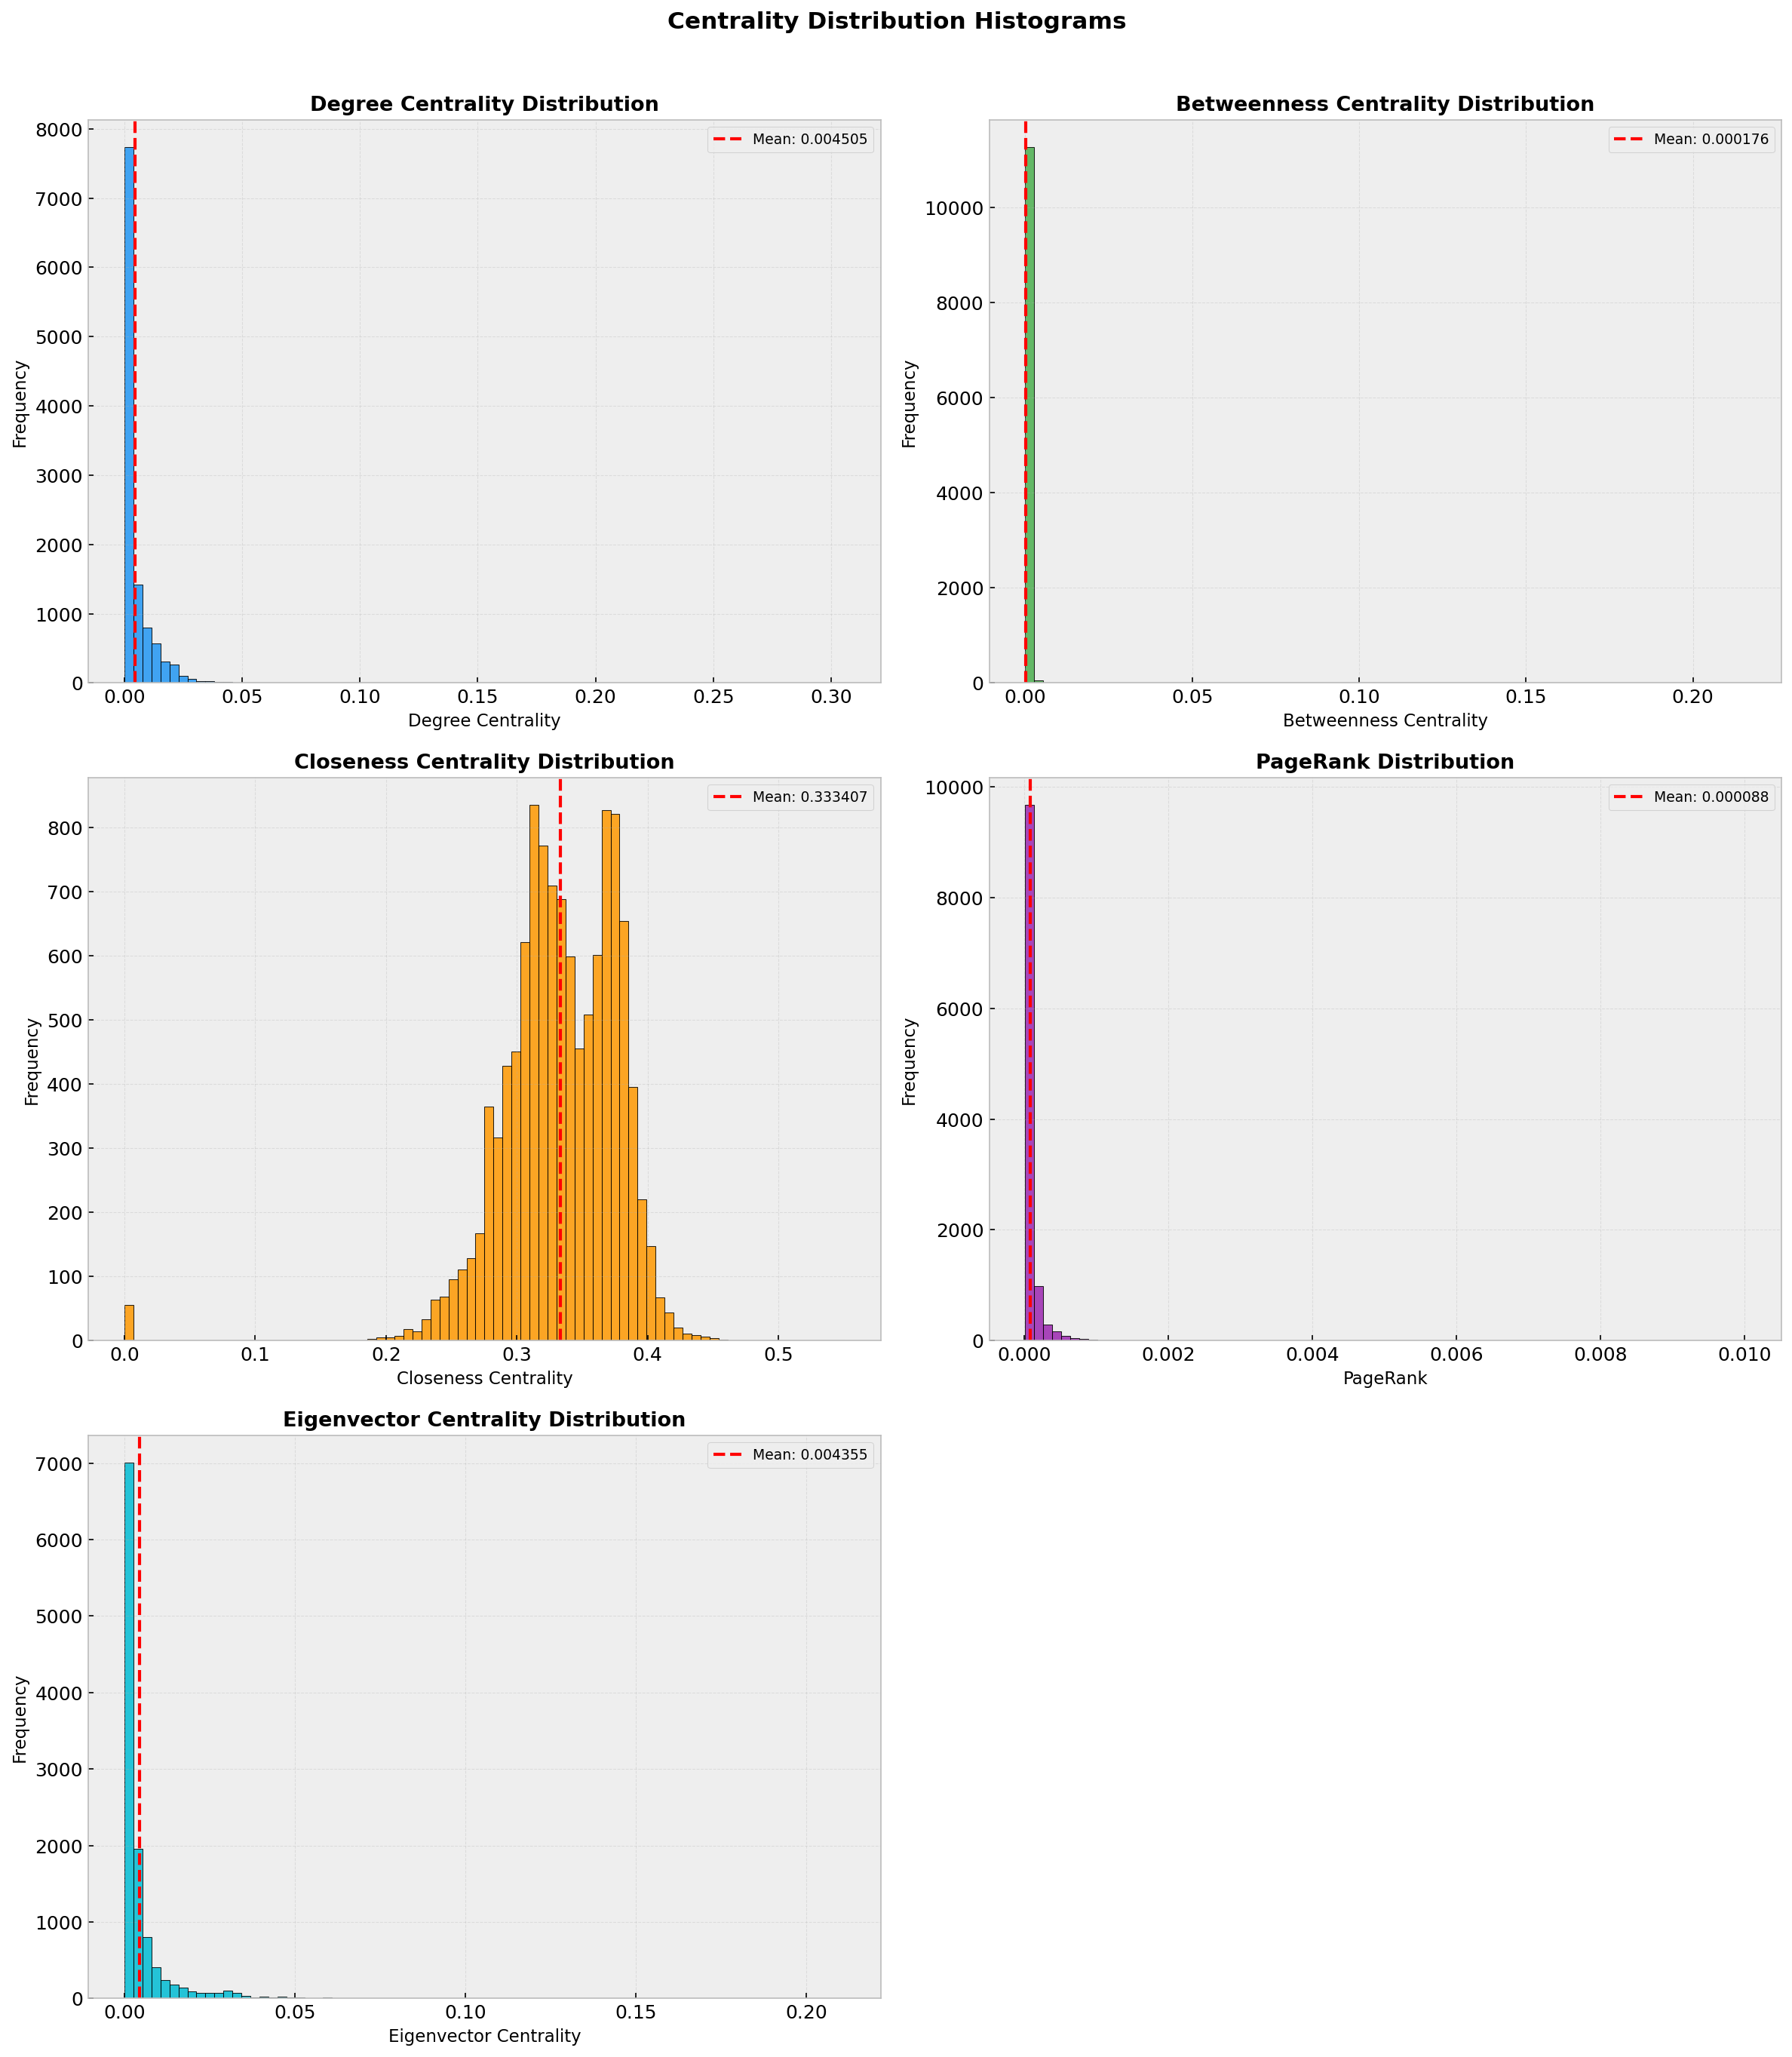
\includegraphics[width=\textwidth]{img-4/centrality-histograms.png}
    \caption{Centrality distribution histograms: Degree (top-left),
             Betweenness (top-right), Closeness (middle-left),
             PageRank (middle-right), Eigenvector (bottom-left).
             Red dashed lines indicate the mean.}
    \label{fig:centrality}
\end{figure}

All five distributions are right-skewed.  Degree, Betweenness, PageRank, and
Eigenvector concentrate the bulk of their mass near zero with long tails toward
the right, characteristic of scale-free networks.  Closeness Centrality is more
bell-shaped and centred around $0.33$, indicating that most nodes in the giant
component have comparable average path lengths.  Eigenvector centrality reveals
nodes that are not just highly connected but connected to other influential nodes,
with influence concentrated in a small elite of articles (max~$=0.2112$, about
$50\times$ the mean).

% ═══════════════════════════════════════════════════════════════════════════
\section{Community Detection}
% ═══════════════════════════════════════════════════════════════════════════

Two community detection algorithms were applied to the undirected cleaned graph:
\textbf{Louvain} (modularity maximisation) and \textbf{Infomap}
(map-equation minimisation via random walks).

\subsection{Louvain Algorithm}

\begin{table}[H]
\centering
\caption{Louvain community detection results.}
\label{tab:louvain}
\begin{tabular}{lr}
\toprule
\textbf{Statistic} & \textbf{Value} \\
\midrule
Modularity              & 0.6504 \\
Number of communities   & 373 \\
Min community size      & 1 \\
Max community size      & 1\,971 \\
Mean community size     & 31.37 \\
Median community size   & 1.0 \\
Std deviation           & 176.52 \\
\bottomrule
\end{tabular}
\end{table}

Louvain achieves a modularity of \textbf{0.6504}, indicating a strong community
structure.  The algorithm identifies 373 communities.  The size distribution
is extremely skewed: the median is 1 (many singleton communities), while the
largest community spans 1\,971 nodes.  The standard deviation ($176.52$) is
more than five times the mean, confirming the imbalance.

\begin{figure}[H]
    \centering
    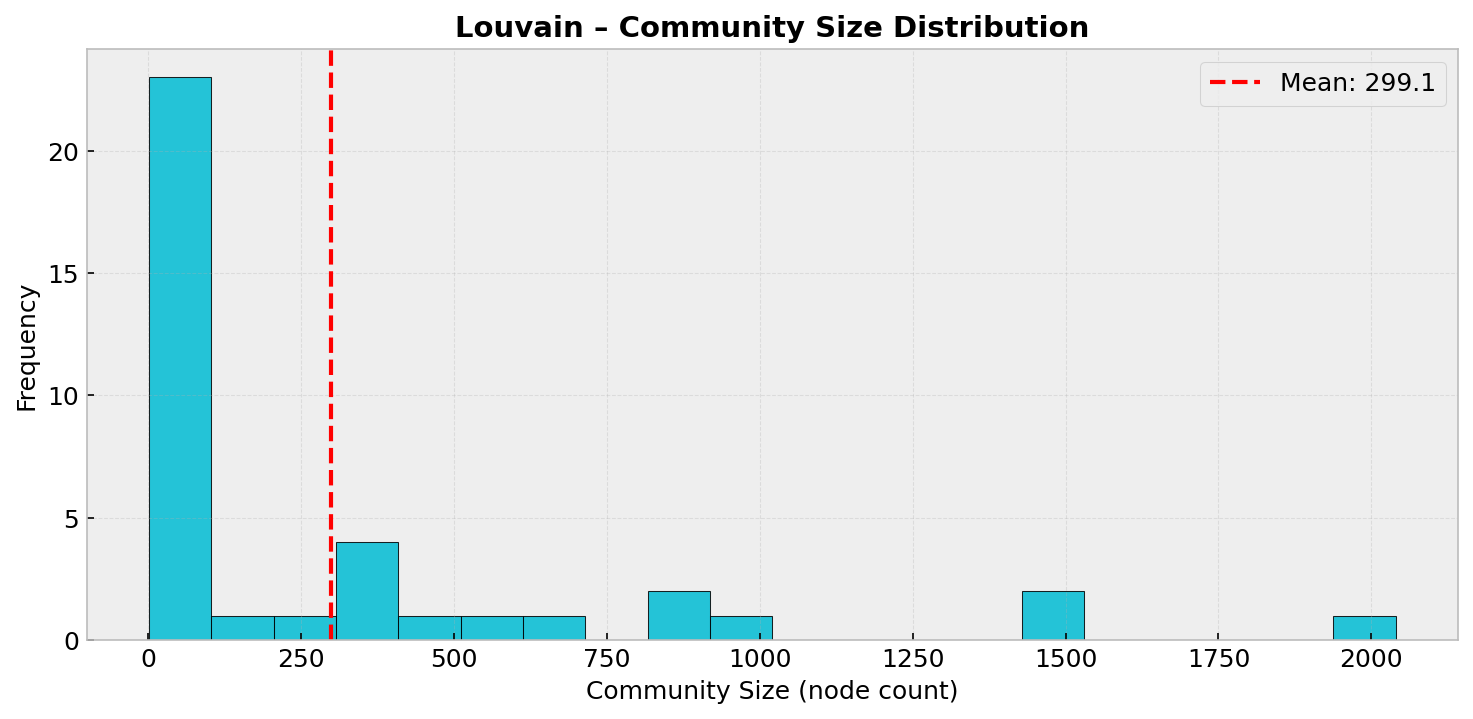
\includegraphics[width=0.85\textwidth]{img-4/community-size-distribution-louvain.png}
    \caption{Louvain community size distribution.  Red dashed line marks the
             mean ($31.4$).}
    \label{fig:louvain}
\end{figure}

Figure~\ref{fig:louvain} confirms the heavy-tailed distribution: the overwhelming
majority of communities have fewer than 50 nodes, while a handful of large
clusters extend the tail past 1\,500 nodes.  This suggests a small number of
broad topical clusters (e.g., ``Machine Learning'', ``Algorithms'') alongside
numerous narrowly-scoped micro-topics.

\subsection{Infomap Algorithm}

\begin{table}[H]
\centering
\caption{Infomap community detection results.}
\label{tab:infomap}
\begin{tabular}{lr}
\toprule
\textbf{Statistic} & \textbf{Value} \\
\midrule
Modularity              & 0.5998 \\
Number of communities   & 596 \\
Min community size      & 1 \\
Max community size      & 837 \\
Mean community size     & 19.63 \\
Median community size   & 1.0 \\
Std deviation           & 73.56 \\
\bottomrule
\end{tabular}
\end{table}

Infomap yields a modularity of \textbf{0.5998}, slightly lower than Louvain.
It discovers 596 communities---roughly $60\%$ more than Louvain.  The maximum
community size drops from 1\,971 to 837, and the mean from 31.37 to 19.63,
indicating that Infomap produces a finer-grained partition.

\begin{figure}[H]
    \centering
    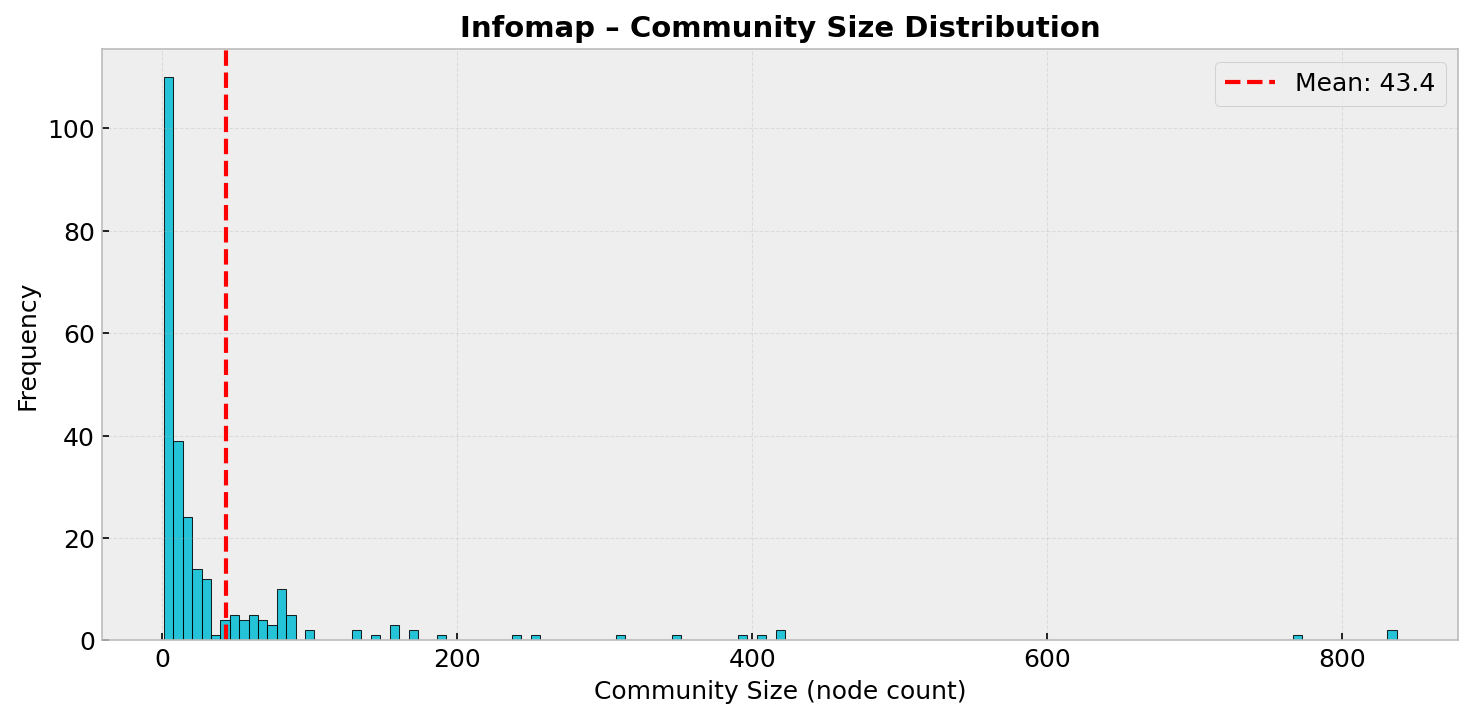
\includegraphics[width=0.85\textwidth]{img-4/community-size-distribution-infomap.png}
    \caption{Infomap community size distribution.  Red dashed line marks the
             mean ($19.6$).}
    \label{fig:infomap}
\end{figure}

Figure~\ref{fig:infomap} shows that Infomap's distribution has a shorter tail
(max~837 vs.\ 1\,971) and more communities in the 10--100 range than Louvain.
Its information-theoretic approach captures tighter flow-based modules where a
random walker tends to stay for extended periods.

\subsection{Louvain vs.\ Infomap Comparison}

\begin{table}[H]
\centering
\caption{Louvain vs.\ Infomap comparison.}
\label{tab:comparison}
\begin{tabular}{lrrrrrrr}
\toprule
\textbf{Algorithm} & \textbf{Modularity} & \textbf{Communities} & \textbf{Min} & \textbf{Max} & \textbf{Mean} & \textbf{Median} & \textbf{Std} \\
\midrule
Louvain & 0.6504 & 373 & 1 & 1\,971 & 31.37 & 1.0 & 176.52 \\
Infomap & 0.5998 & 596 & 1 & 837   & 19.63 & 1.0 & 73.56  \\
\bottomrule
\end{tabular}
\end{table}

Key differences:
\begin{itemize}
    \item \textbf{Modularity:} Louvain achieves a higher modularity ($0.6504$
          vs.\ $0.5998$), as it directly optimises this metric.  Infomap
          optimises a different (information-theoretic) objective that may
          capture more nuanced flow patterns.
    \item \textbf{Granularity:} Infomap produces $\sim$$60\%$ more communities.
          Its largest community ($837$~nodes) is less than half the size of
          Louvain's largest ($1\,971$~nodes), providing a more fine-grained
          decomposition.
    \item \textbf{Size distribution:} Both yield many singleton communities
          (median~$=1$), but Louvain's standard deviation is more than twice
          that of Infomap ($176.52$ vs.\ $73.56$), indicating a more uneven
          split with a few very large super-communities.
    \item \textbf{Interpretation:} Louvain groups nodes by maximising internal
          edge density relative to a null model.  Infomap's random-walk
          approach detects regions where information flow is self-contained,
          which may better capture thematic sub-topics.
\end{itemize}

% ═══════════════════════════════════════════════════════════════════════════
\section{Community Similarity Analysis}
% ═══════════════════════════════════════════════════════════════════════════

To evaluate whether the structural communities correspond to semantically
coherent groups, we compute the cosine similarity of node embeddings for
intra-community and inter-community undirected edges.

\begin{figure}[H]
    \centering
    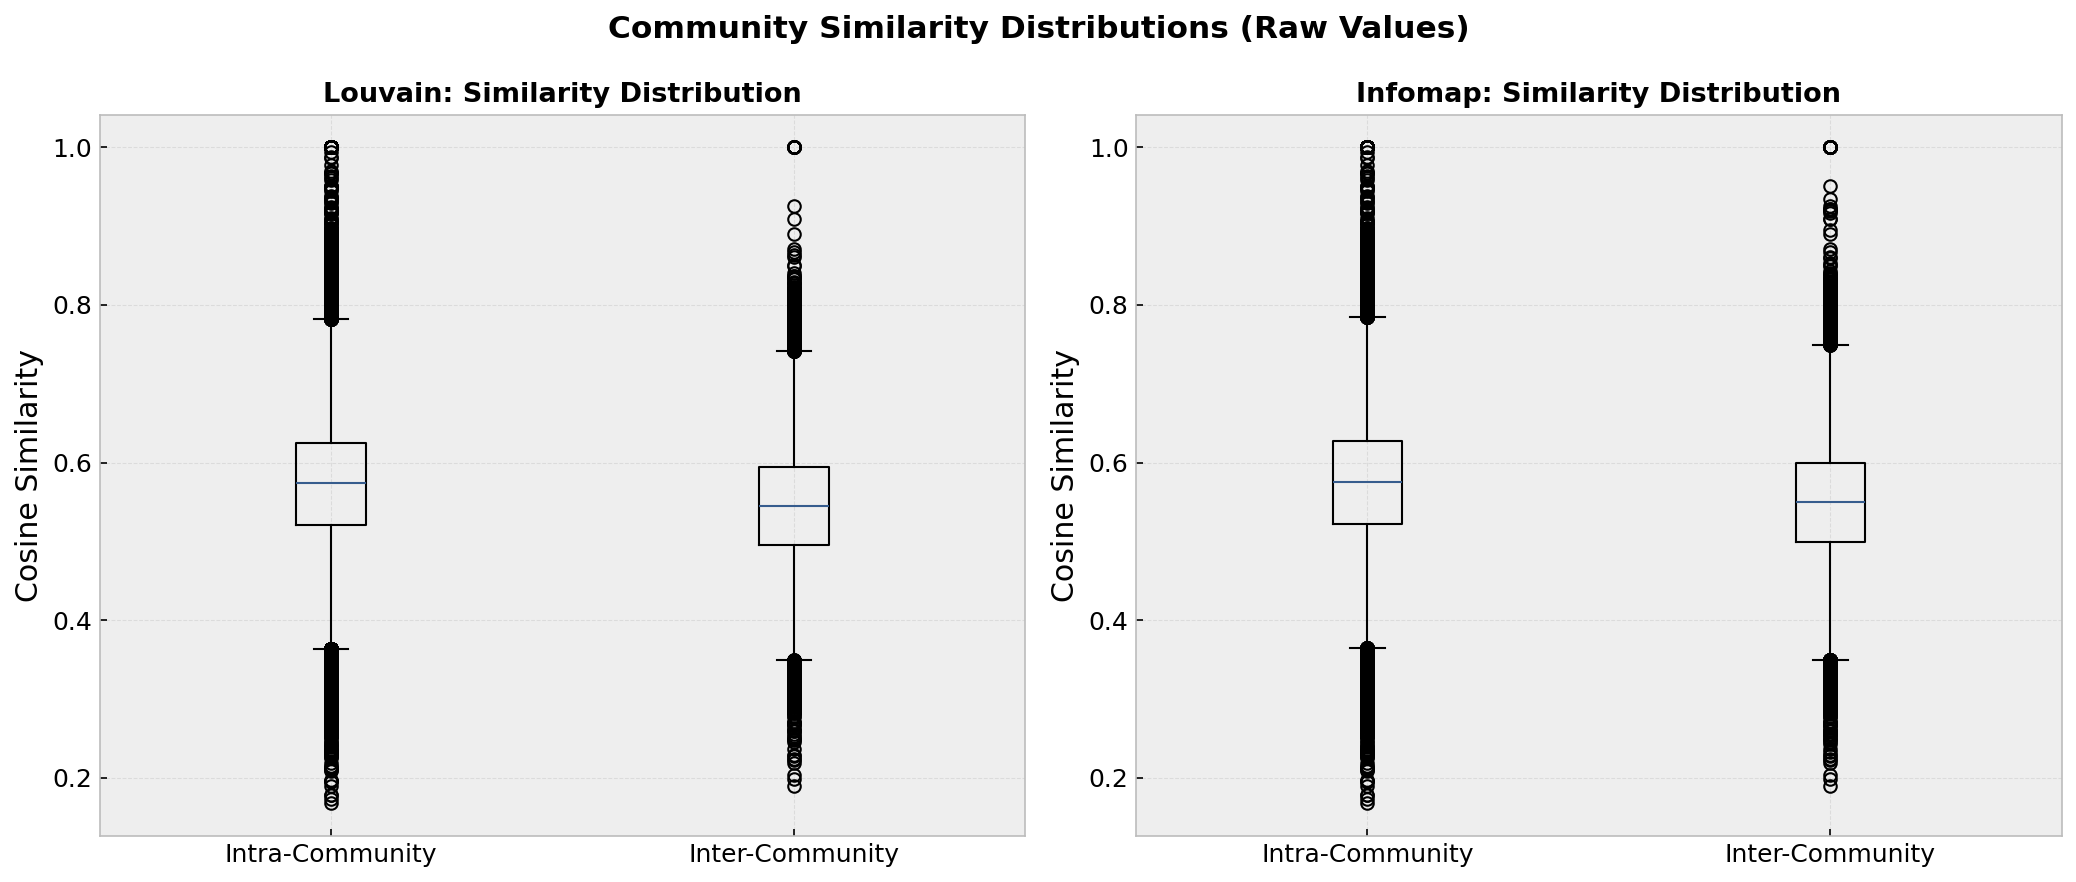
\includegraphics[width=0.85\textwidth]{img-4/similarity-distributions.png}
    \caption{Box plots of intra-community vs.\ inter-community cosine
             similarity: Louvain (left) and Infomap (right).}
    \label{fig:sim_dist}
\end{figure}

\begin{table}[H]
\centering
\caption{Average cosine similarity: Intra-community vs.\ inter-community.}
\label{tab:sim_comparison}
\begin{tabular}{lccc}
\toprule
\textbf{Algorithm} & \textbf{Intra-Community} & \textbf{Inter-Community} & \textbf{Difference} \\
\midrule
Louvain & 0.5795 & 0.5481 & +0.0314 \\
Infomap & 0.5726 & 0.5481 & +0.0245 \\
\bottomrule
\end{tabular}
\end{table}

Both algorithms confirm that nodes within the same community share a higher
average cosine similarity than nodes in different communities.  Louvain shows a
slightly larger intra-inter gap ($+0.0314$) than Infomap ($+0.0245$), consistent
with its higher modularity score.  The difference is subtle but statistically
meaningful, supporting the hypothesis that structural community detection
successfully groups topically related articles.

% ═══════════════════════════════════════════════════════════════════════════
\section{Node Degree vs.\ Average Neighbor Similarity}
% ═══════════════════════════════════════════════════════════════════════════

To investigate whether a node's topological importance (degree) correlates with
the semantic similarity of its neighbours, nodes were grouped into degree ranges
and the average cosine similarity of their neighbours was computed.

\begin{figure}[H]
    \centering
    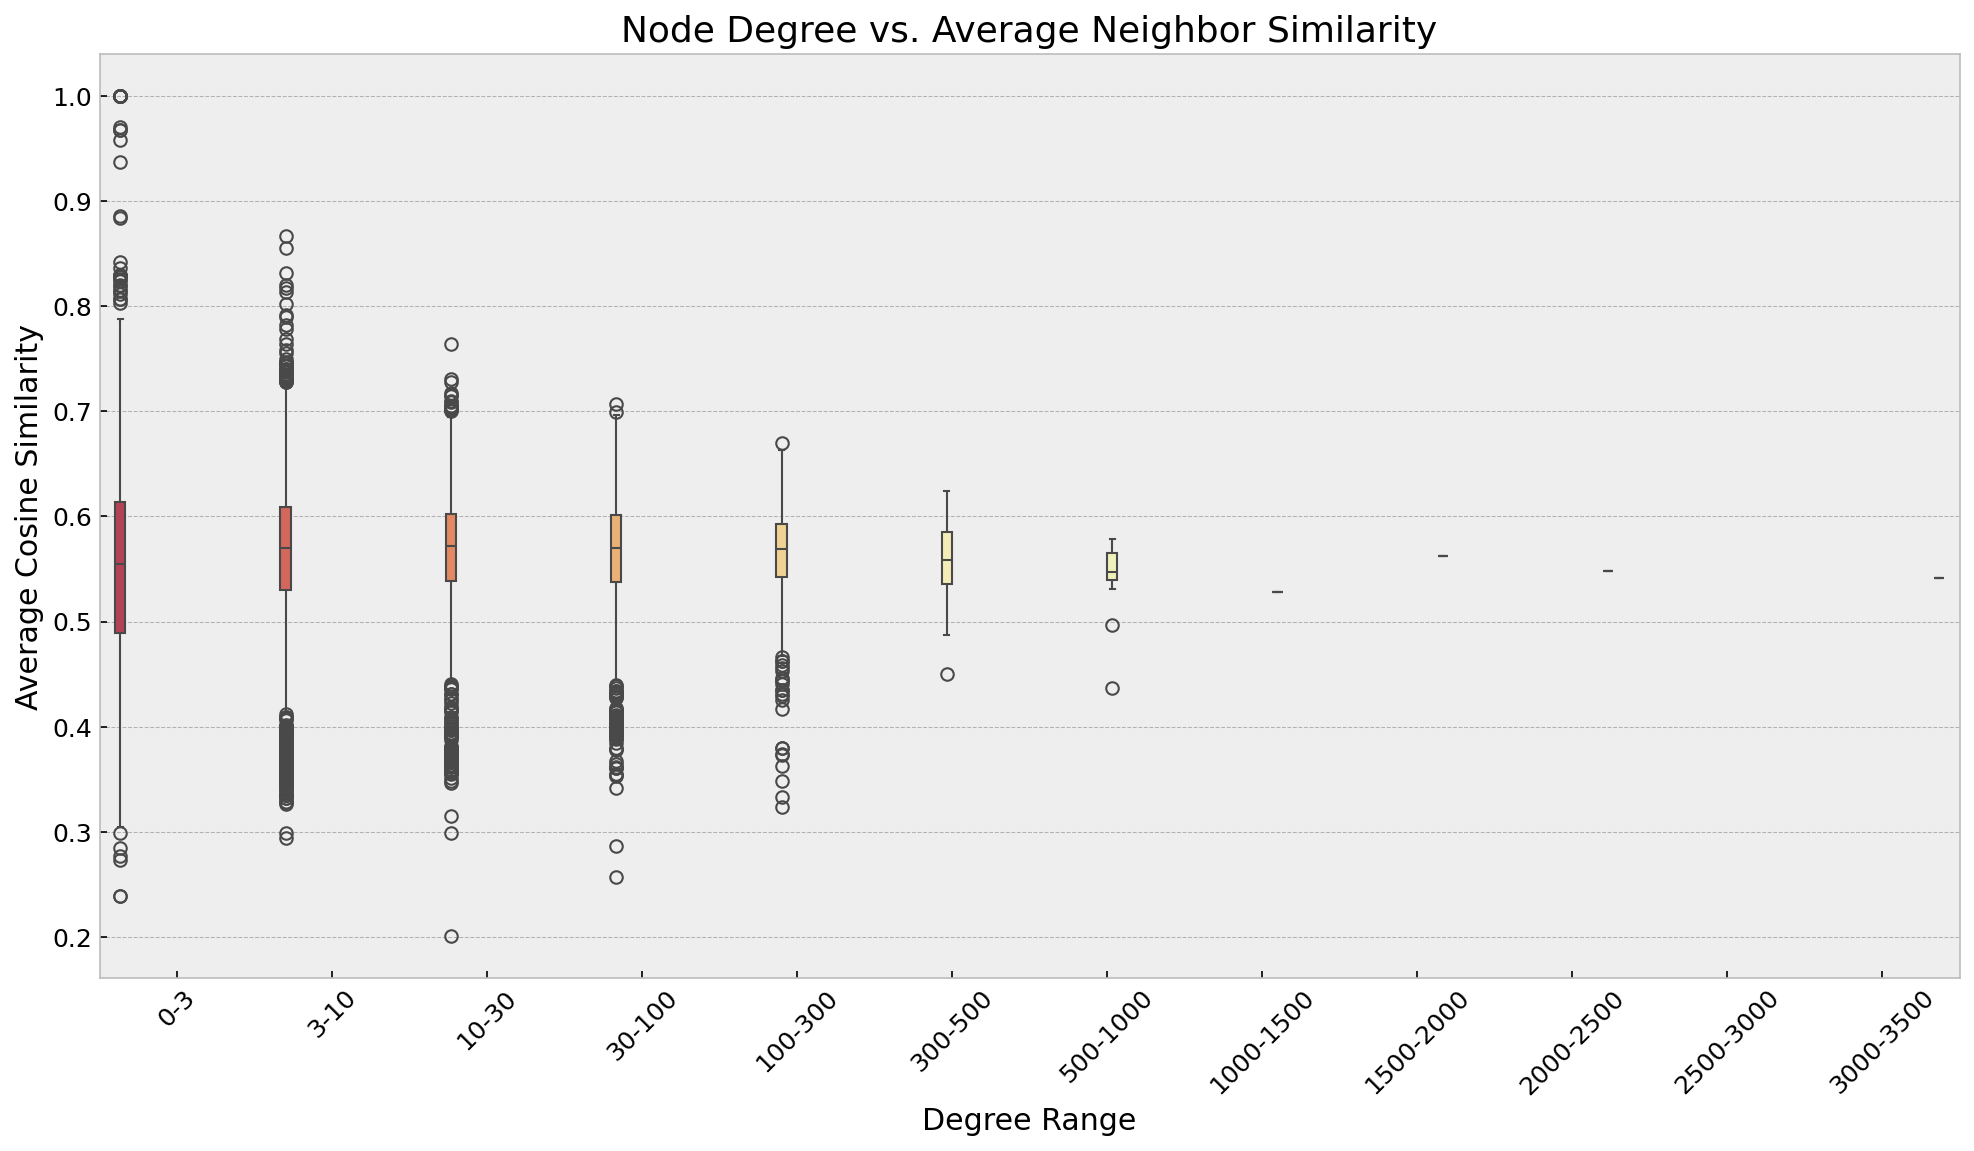
\includegraphics[width=0.85\textwidth]{img-4/degree-vs-similarity.png}
    \caption{Node degree range vs.\ average neighbour cosine similarity
             (box plot).}
    \label{fig:degree_sim}
\end{figure}

Figure~\ref{fig:degree_sim} illustrates that nodes with very high degrees
($\geq$1\,000) tend to have neighbour similarity distributions that converge
toward the global mean, acting as generalist hubs that connect to diverse topics.
In contrast, low-degree nodes (degree~$<$30) show higher variance in neighbour
similarity, with some occupying highly specific, semantically tight-knit niches
and others being generalists.  The box plot also reveals that the interquartile
range narrows progressively with increasing degree, confirming the
variance-reduction effect of hub nodes.

% ═══════════════════════════════════════════════════════════════════════════
\section{Appendix A: Statistical Tests for Community Similarity}
% ═══════════════════════════════════════════════════════════════════════════

To formally test whether the observed difference between intra-community and
inter-community similarity is statistically significant, an independent samples
$t$-test was conducted for both Louvain and Infomap community assignments.

\subsection{Louvain T-Test Results}

\begin{table}[H]
\centering
\caption{Louvain community similarity: T-test results.}
\label{tab:louvain_ttest}
\begin{tabular}{lr}
\toprule
\textbf{Metric} & \textbf{Value} \\
\midrule
Intra-community edges (n) & 159\,552 \\
Inter-community edges (n) & 56\,571 \\
Intra-community mean similarity & 0.5729 \\
Inter-community mean similarity & 0.5435 \\
t-statistic & 68.1973 \\
p-value & $<$0.0001 \\
Cohen's $d$ effect size & 0.345 \\
Significant (p $<$ 0.05) & Yes \\
\bottomrule
\end{tabular}
\end{table}

\subsection{Infomap T-Test Results}

\begin{table}[H]
\centering
\caption{Infomap community similarity: T-test results.}
\label{tab:infomap_ttest}
\begin{tabular}{lr}
\toprule
\textbf{Metric} & \textbf{Value} \\
\midrule
Intra-community edges (n) & 138\,656 \\
Inter-community edges (n) & 77\,467 \\
Intra-community mean similarity & 0.5748 \\
Inter-community mean similarity & 0.5480 \\
t-statistic & 67.8098 \\
p-value & $<$0.0001 \\
Cohen's $d$ effect size & 0.311 \\
Significant (p $<$ 0.05) & Yes \\
\bottomrule
\end{tabular}
\end{table}

\subsection{Summary and Interpretation}

\begin{table}[H]
\centering
\caption{Community similarity t-test summary for both algorithms.}
\label{tab:ttest_summary}
\begin{tabular}{lcccccc}
\toprule
\textbf{Algorithm} & \textbf{Intra N} & \textbf{Inter N} & \textbf{Intra Mean} & \textbf{Inter Mean} & \textbf{t-stat} & \textbf{p-value} \\
\midrule
Louvain & 159\,552 & 56\,571 & 0.5729 & 0.5435 & 68.20 & $<$0.0001 \\
Infomap & 138\,656 & 77\,467 & 0.5748 & 0.5480 & 67.81 & $<$0.0001 \\
\bottomrule
\end{tabular}
\end{table}

Both Louvain and Infomap yield highly significant t-statistics ($t > 67$, $p < 0.0001$),
confirming that the observed difference between intra-community and inter-community
similarity is not due to random chance.  However, the effect size (Cohen's $d \approx 0.31$--$0.35$)
is small to medium, indicating that while the difference is real, the practical
magnitude of the separation is modest.  This aligns with the visual observation
from the box plots: the two distributions overlap considerably, with intra-community
similarity being only marginally higher on average.

\subsection{Node Count Annotations for Degree vs.\ Similarity Box Plot}

Figure~\ref{fig:degree_sim} was annotated with the number of nodes in each degree
range to provide additional context.

\begin{figure}[H]
    \centering
    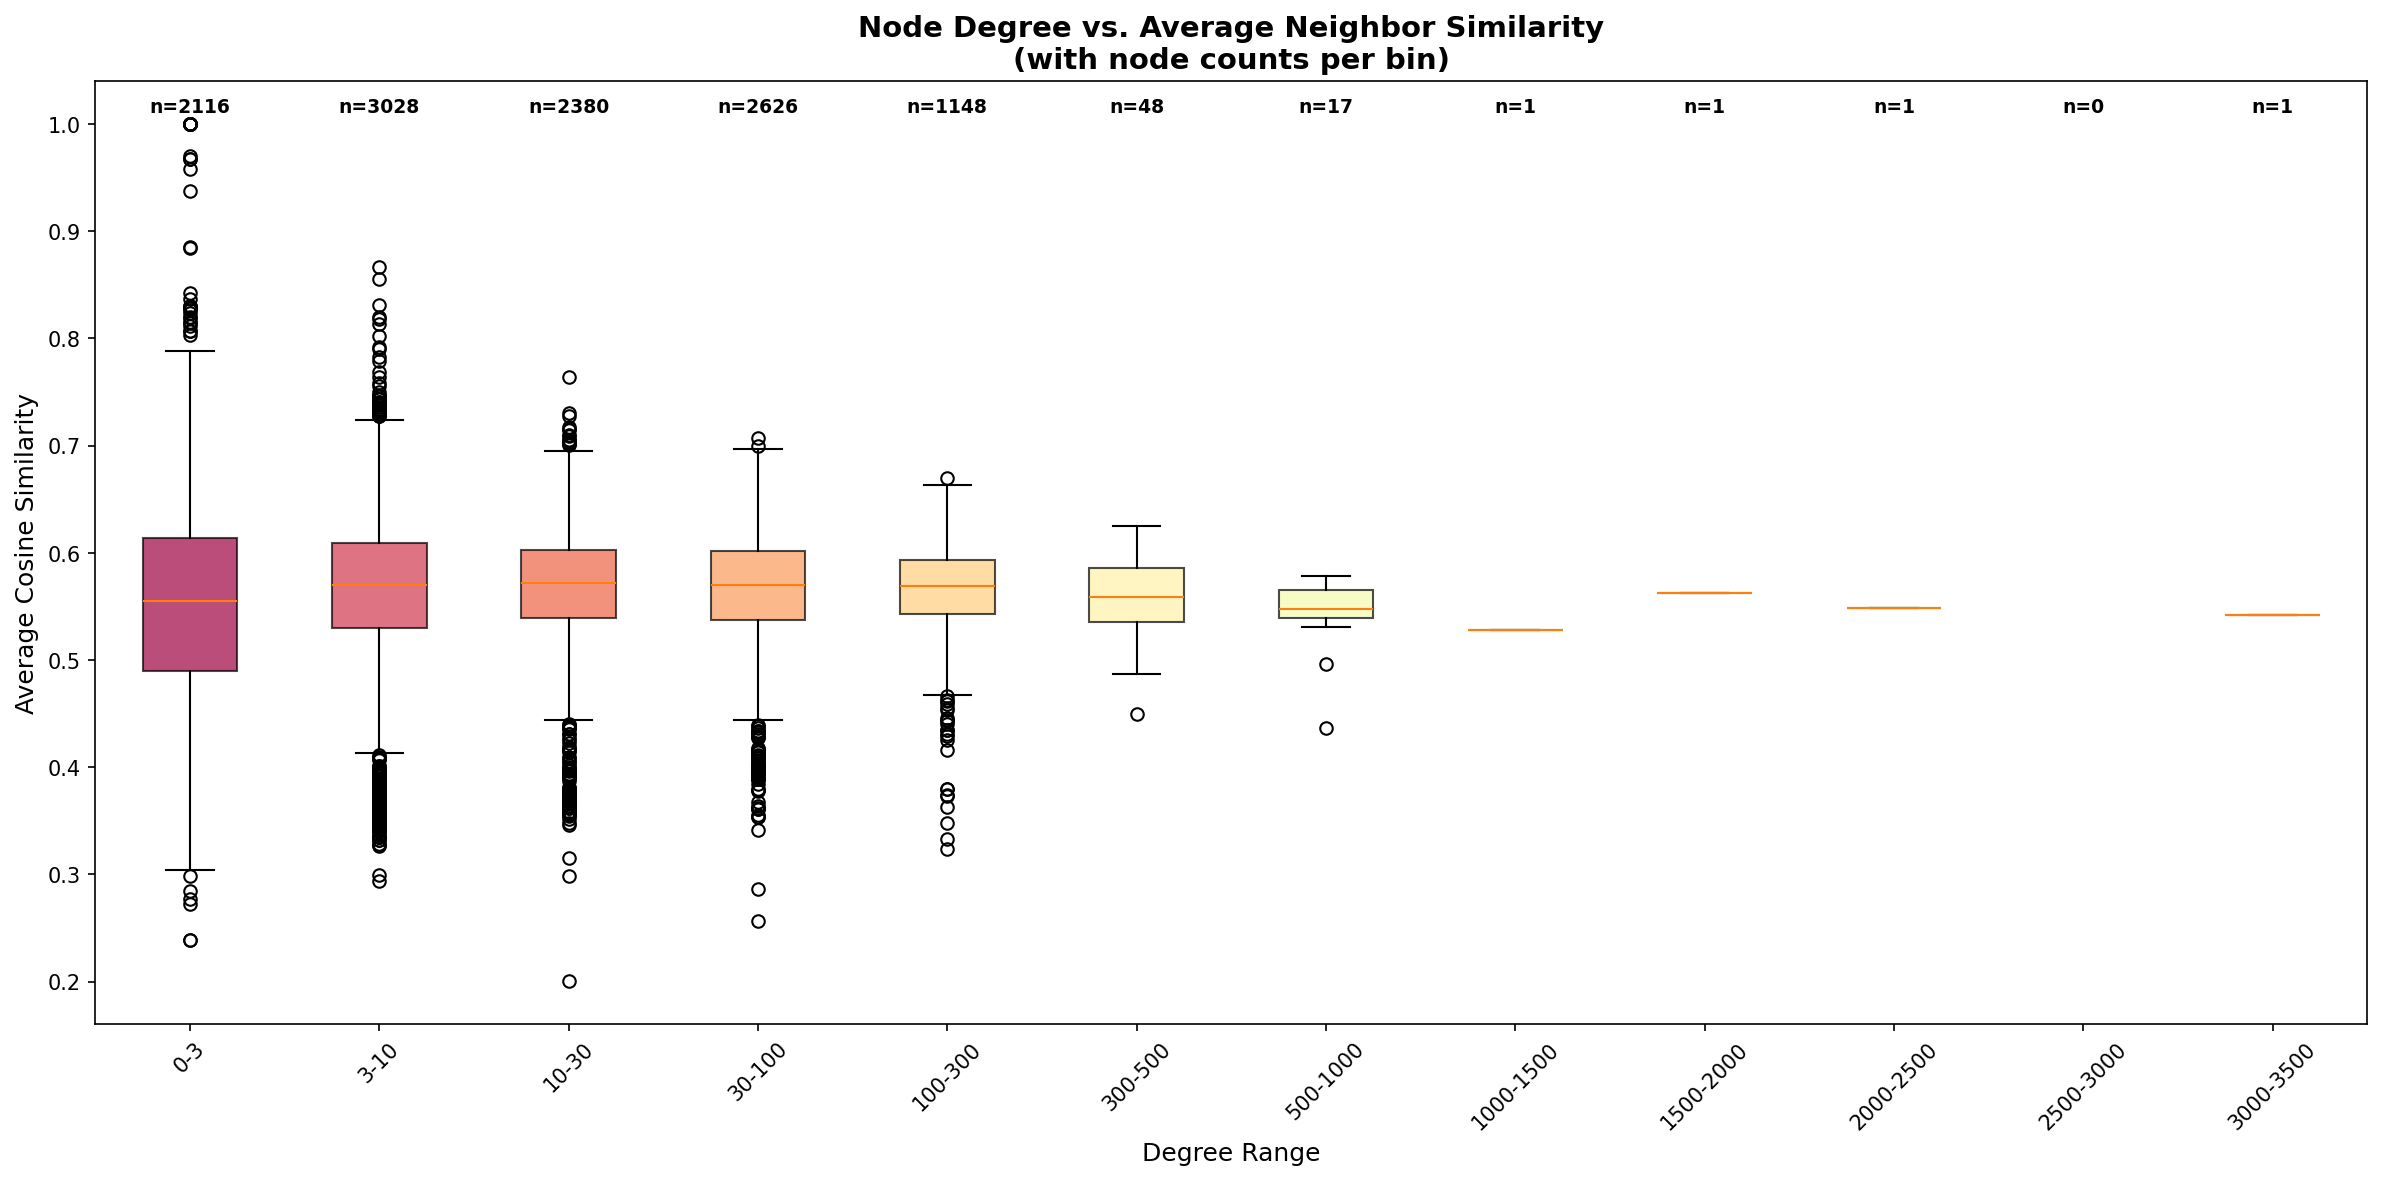
\includegraphics[width=0.85\textwidth]{img-4/degree-vs-similarity-annotated.png}
    \caption{Node degree range vs.\ average neighbour cosine similarity
             (annotated with node counts per bin).}
    \label{fig:degree_sim_annotated}
\end{figure}

\begin{table}[H]
\centering
\caption{Node counts per degree bin for Figure~\ref{fig:degree_sim_annotated}.}
\label{tab:degree_bin_counts}
\begin{tabular}{lr}
\toprule
\textbf{Degree Range} & \textbf{Node Count} \\
\midrule
0--3 & 2\,116 \\
3--10 & 3\,028 \\
10--30 & 2\,380 \\
30--100 & 2\,626 \\
100--300 & 1\,148 \\
300--500 & 48 \\
500--1000 & 17 \\
1000--1500 & 1 \\
1500--2000 & 1 \\
2000--2500 & 1 \\
2500--3000 & 0 \\
3000--3500 & 1 \\
\bottomrule
\end{tabular}
\end{table}

The degree distribution is heavily right-skewed: the vast majority of nodes
(10\,150 out of 11\,367) fall in the 0--100 degree range, while fewer than 70
nodes have degree exceeding 300.  This confirms the scale-free nature of the
network and explains why high-degree bins have limited sample sizes for
similarity statistics.

% ═══════════════════════════════════════════════════════════════════════════
\section{Conclusion}
% ═══════════════════════════════════════════════════════════════════════════

Phase 4 of the Custom-WikiCS analysis demonstrates that:

\begin{itemize}
    \item Removing 334 isolated nodes yields a cleaner structural baseline of
          11\,367 active nodes without altering any edge statistics.
    \item The degree distribution follows a power-law--like pattern on log--log
          axes, consistent with a scale-free information network.
    \item The network is disassortative ($r=-0.0918$): hub articles tend to link
          to low-degree articles rather than to other hubs.
    \item Linked pairs are topically more similar than random pairs across all
          three embedding metrics (cosine~$+0.14$, Pearson~$+0.14$,
          Euclidean~$-0.14$), confirming the topic-link relationship.
    \item Local transitivity is high for many nodes (mean CC~$=0.4660$) while
          global transitivity is lower ($0.2623$), indicating dense local
          neighbourhoods within a sparser global structure.
    \item No significant correlation exists between local transitivity and
          cosine similarity at the edge level, indicating that topological
          clustering and semantic similarity are largely orthogonal properties.
    \item Louvain (modularity~$0.6504$) and Infomap (modularity~$0.5998$) both
          identify meaningful community structure; Louvain produces fewer,
          larger communities while Infomap yields finer-grained partitions.
    \item Intra-community edges are consistently more similar than
          inter-community edges for both algorithms (Louvain: $t=68.20$, Infomap:
          $t=67.81$, $p<0.0001$), confirming that the difference is statistically
          significant though small in practical effect (Cohen's $d\approx0.31$--$0.35$).
    \item High-degree hub nodes act as generalist connectors with average
          neighbour similarity converging to the global mean, while low-degree
          nodes exhibit higher variance, reflecting both specialist niches and
          generalist peripheral positions.
\end{itemize}

These findings collectively confirm that the Custom-WikiCS graph possesses a
rich, multi-layered structure: a scale-free topology with disassortative mixing,
dense local clustering, meaningful modular decomposition, and a clear
topical coherence of hyperlinks that aligns with the embedding space.

\end{document}
